\documentclass[cn,11pt,chinese]{elegantbook}

\usepackage[all]{xy}
\usepackage{amsmath}
\usepackage{asymptote}
\usepackage{subfig}
\usepackage{graphicx}



\newcount\mycount
%\def\ConvColor{rgb:yellow,5;red,2.5;white,5}
%\def\ConvReluColor{rgb:yellow,5;red,5;white,5}
%\def\PoolColor{rgb:red,1;black,0.3}
%\def\FcColor{rgb:blue,5;red,2.5;white,5}
%\def\FcReluColor{rgb:blue,5;red,5;white,4}
%\def\SoftmaxColor{rgb:magenta,5;black,7}

%\newtheorem{lemma}{法则}



% title info
\title{数学书籍汇总}
\subtitle{读书笔记}

% bio info
\author{虞朝阳}
\institute{西北工业大学}
%\date{\today}

% extra info
\version{1.00}
\equote{Wir m\"ussen wissen, wir werden wissen. (我们必须知道,我们必将知道) - David.Hilbert}
%\logo{logo.png}
\cover{cover.jpg}

\begin{document}

\maketitle


\chapter*{前言}
\addcontentsline{toc}{chapter}{Preface}
\markboth{Preface}{}
这里收集了大量的数学书籍,大部分都是比较经典的,包含了代数,几何,分析,组合数学等各个分支的数学书籍。原著如果是英文的,将会被翻译成中文,所以收集整理的进度上不可能会太快。

我希望最终能形成一本书:尽早引入一些抽象代数的概念,能够尽量给出各种应用。初步设想从集合的一些基础知识出发,引入基本的群环域的概念,从自然数出发,构造整数,然后引入一些数论的基础知识,进一步构造有理数,实数,复数,然后开始讨论一些微积分。从线性代数和几何角度,再次出发。



\tableofcontents
\mainmatter
\hypersetup{pageanchor=true}

% add preface chapter here if needed
\part{代数}
\chapter{近世代数概论}
《近世代数概论》的作者是G.伯克霍夫和S.麦克莱恩。参考:\cite{surveyofmodernalgebra1979}。

\section{整数}\label{section001}
\subsection{交换环, 整环}
近世代数第一次揭示了数学系统的多变性和丰富性。本书从最基本也是最古老的正整数系统(整数系统,记为$\mathbb{Z}$)开始。

首先假定加法和乘法的八个公设,这些公设不仅对整数成立,而且对于很多数学系统都成立,例如所有有理数,所有实数,所有复数,所有多项式,任意已知区间上的连续函数。

\begin{definition}{交换环}{ring} 
设$R$是由元素$a,b,c,\cdots$组成的集合,在$R$上定义了任意两个元素$a$与$b$的和$a+b$及积$ab$.如果下列公设(i)-(viii)成立,那么$R$称为交换环:
\begin{enumerate}
\item[(i)] 封闭性. 若$a$, $b \in R$, 则$a+b \in R$,$ab \in R$.
\item[(ii)] 唯一性. 若$R$中$a=a'$且$b=b'$,则$a+b=a'+b'$以及$ab=a'b'$。
\item[(iii)]交换律. 对$R$中一切$a$与$b$,
\[
a+b=b+a,\quad ab=ba.
\]
\item[(iv)]对一切$a,b,c \in R$,
\[
\begin{aligned}
a + (b + c) &= (a+b)+c, \\
a(bc) &= (ab)c.
\end{aligned}
\]
\item[(v)]分配律. 对一切$a,b,c \in R$,
\[
a(b + c)=ab + ac. 
\]
\item[(vi)]零. $R$中包含元素$0$,使得对于一切$a \in R$, 
\[
a + 0 = a.
\]
\item[(vii)]单位元素. $R$中包含元素$1 \neq 0$,使得对于一切$a \in R$,
\[
a1=a.
\]
\item[(viii)]加法逆元素.对于每个$a \in R$,方程
\[
a + x = 0
\]
在$R$中有解$x$. $x$称为$a$的逆元素,并记为$-a$.
\end{enumerate}
\end{definition}

首先定义中的$1 \neq 0$,排除只包含一个元素$0$的情形。其次,$0$和$1$其实起着相似的作用,所以可以分别称为加法和乘法单位元。第三,交换中只保证了加法存在逆元素,对于乘法没有这个保证,这样一来,在整数集合$\mathbb{Z}$中,$c \neq 0$,且$ca=cb$,则必有$a=b$,这个结论对于一般的交换环不成立(例如区间上全体实函数组成的集合)。为此引入整环的概念。
\begin{definition}{整环}{integerRing} 
满足下面附加公设的交换环是整环:
\begin{enumerate}
\item[(ix)] 消去律. 若$c \neq 0$且$ca=cb$, 则$a=b$.
\end{enumerate}
\end{definition}

整环并不保证每个非零元素存在乘法逆元素。不过后面会证明$1$是有乘法逆元素的($1$自身),$-1$也有乘法逆元素$-1$。

这里应该多举一些交换环和整环的例子。

集合$\mathbb{Z}[\sqrt{2}] = \{a+b\sqrt{2} | a,b \in \mathbb{Z}\}$是一个整环,$a+b\sqrt{2}=c+d\sqrt{2}$当且仅当$a=c$且$b=d$,加法和乘法分别定义为:
\[
\begin{aligned}
(a + b\sqrt{2}) + (c + d\sqrt{2}) &= (a+c) + (b+d)\sqrt{2}, \\
(a + b\sqrt{2})(c + d\sqrt{2})&=(ac+2bd)+(ad+bc)\sqrt{2}.
\end{aligned}
\]

\subsection{交换环的基本性质}
当我们想要得到对于整个代数系统都正确的结论时,必须多加小心,我们必须确信,所有的证明只用到明显列出的公设和一般逻辑法则,其中最基本的逻辑法则是相等关系的三个基本定律:对一切$a$,$b$,$c$有
\begin{itemize}
\item 自反律 $a=a$.
\item 对称律 若$a=b$,则$b=a$.
\item 传递律 若$a=b$且$b=c$,则$a=c$.
\end{itemize}

下面任意交换环都成立的一些基本法则。 证明的时候只是需要注意只能使用公设或者前面证明的结论。这里省略,参考书本。

\begin{corollary}{法则1}{rule1}
对一切$a,b,c \in R$,有
\[
(a+b)c = ac + bc.
\]
\end{corollary}

这条法则可称为右分配律,可与公设(v)对比,公设(v)是左分配律。

\begin{corollary}{法则2}{rule2}
对一切$a \in R$,$0+a=a$且$1a=a$。
\end{corollary}

\begin{corollary}{法则3}{rule3}
如果$z \in R$满足:对一切$a \in R$,$a+z=a$,那么$z=0$。
\end{corollary}
这个法则说明加法单位元素0的唯一性。

\begin{corollary}{法则4}{rule4}
对一切$a, b, c \in R$成立:由$a+b=a+c$,可推出$b=c$。
\end{corollary}
这个法则称为加法消去律。

\begin{corollary}{法则5}{rule5}
对一切$a \in R$,存在唯一的$x \in R$满足$a+x=0$。
\end{corollary}
公设(viii)只保证了存在性,这个法则说明唯一性。

\begin{corollary}{法则6}{rule6}
对一切$a, b \in R$,存在唯一的$x \in R$使得$a+x=b$。
\end{corollary}
这个法则说明减法是可能的而且差是唯一的。

\begin{corollary}{法则7}{rule7}
对一切$a \in R$,$a \cdot 0 = 0 = 0 \cdot a$。
\end{corollary}

\begin{corollary}{法则8}{rule8}
如果$u \in R$满足:对一切$a \in R$,$au=a$,那么$u=1$。
\end{corollary}
这个法则说明乘法单位元素1的唯一性。

\begin{corollary}{法则9}{rule9}
对一切$a, b \in R$,$(-a)(-b)=ab$。
\end{corollary}

特别的有$(-1)(-1)=1$。这个证明起来稍微麻烦一点,不过只需要注意到$-a$,$-b$的定义,一步一步来还是可以得到的。只需要考虑
\[
[ab + a(-b)] + (-a)(-b) = ab + [a(-b) + (-a)(-b)]
\]
即可。中间的$a(-b)$可以换成$(-a)b$。另外需要使用法则7。

还有一条基本的代数定律是用于解二次方程的:若$ab=0$,则或者$a=0$或者$b=0$。遗憾的是,这个断语不是对一切交换环成立的。但是在任意的整环$D$中成立(可以根据乘法消去律证明)。反之,在任意交换环中,从这个断语可以得到消去律。若$a \neq 0$,从$ab=ac$有$ab-ac=a(b-c)=0$,可得$b-c=0$从而$b=c$.于是我们有:
\begin{theorem}{}{theorem1}
在交换环中,乘法消去律等价于“非零元素之积不为零”这个命题。
\end{theorem}
这里所谓“非零元素之积不为零”这个命题,可以用符号表示为:$a \neq 0$,$b \neq 0$,则必有$ab \neq 0$。我们把满足$ab=0$的非零元素$a$,$b$称为零因子。因此交换环中的消去律等价于“$R$中不包含零因子”。

前面提到$\mathbb{Z}[\sqrt{2}]$是整环,需要证明在$\mathbb{Z}[\sqrt{2}]$中成立消去律,这个可以使用这个定理来完成。证明过程参考书本,需要注意,这里需要用到结论$\sqrt{2}$不是有理数,也就是不能表示为$a/b$的形式,这里$a, b$是整数。

如果承认$\sqrt{2}$是实数,并且承认所有实数的集合构成整环,那么借助于子整环的概念可以非常容易证明$\mathbb{Z}[\sqrt{2}]$是整环。
\begin{definition}{子整环}{defSubIntegerRing}
整环$D$的子整环是$D$的子集,它对于同一种加法和乘法运算也是整环。
\end{definition}

子集$S$是子整环的充分必要条件是:$S$包含0和1;$S$包含其中任意元素$a$的加法逆元素;$S$包含其中任意两个元素$a$与$b$的和$a+b$以及积$ab$。换成集合语言,可以描述如下:
\begin{itemize}
\item $0 \in S$, $1 \in S$;
\item 对任意$a \in S$,必有$-a \in S$;
\item 对任意$a, b \in S$,有$a + b \in S$,$ab \in S$。
\end{itemize}

\subsection{有序整环的性质}\label{subsection00103}
所有整数组成的环$\mathbb{Z}$在数学中起着独特的作用,因此我们将研究它的特殊性质。乘法交换律和消去律仅仅是其中两个,许多其他性质都来源于整数有可能被排成通常的次序:
\[
\cdots,-4,-3,-2,-1,0,1,2,3,4,\cdots
\]
这个次序常用关系$a<b$表示。关系$a<b$成立当且仅当差$b-a$为正整数。假设正整数$1,2,3,\cdots$集合的下列三个性质作为公设。
\begin{itemize}
\item 加法律 两个正整数的和是正整数。
\item 乘法律 两个正整数的积是正整数。
\item 三分律 对于已知整数$a$,下面三种情况中有且仅有一个成立:或者$a$为正整数,或者$a=0$,或者$-a$为正整数。
\end{itemize}

请注意,这里相当于根据这三个公设定义了正整数集合,也就是只要$\mathbb{Z}$的子集$\mathbb{Z}^+$满足这三个公设的就可以作为$\mathbb{Z}$的正整数集合。按照通常的加法,乘法,应该和我们以前学到的是一致的。有必要给这样的整环一个单独的名称。

\begin{definition}{有序整环}{defOrderedIntegerRing}
如果整环$D$中存在某些被称为正元素的元素,它们满足类似于上面对整数指出的加法,乘法和三分律这三个公设,那么称$D$为有序整环。
\end{definition}

明显,整数环$\mathbb{Z}$,有理数环$\mathbb{Q}$,实数环$\mathbb{R}$都是有序整环。所有复数构成的集合是整环,但是无法定义类似整数的序关系,不是有序整环。

\begin{theorem}{}{theorem2}
在任意有序整环中,一切非零元素的平方都是正的。
\end{theorem}

证明使用三分律以及前面的法则9即可。注意所谓平方,意指$a^2 = a \cdot a$。

由此定理,立即可以得到$1=1^2$是正的。从而可以证明在有序整环中$x^2+1=0$无解,也说明所有复数无法构成有序整环。

\begin{definition}{大于,小于关系}{defLess}
在有序整环中,$a<b$和$b>a$这两个等价的说法都意味着$b-a$是正的,还有$a \le b$的意思是$a<b$或者$a=b$。
\end{definition}
根据这个定义,正元素$a$可以描述为大于零的元素,元素$b<0$称为负元素。从定义还可以得出“小于关系”的传递律:
\begin{itemize}
\item 传递律 若$a < b$且$b<c$,则$a<c$。
\end{itemize}

证明直接使用定义以及加法律即可。事实上,根据定义以及正元素的三个公设,正好对应到不等式的三个性质:
\begin{itemize}
\item 不等式两边同时加上一个元素 若$a < b$,则$a+c < b+c$。
\item 不等式两边同时乘以一个正元素 若$a < b$且$c > 0$,则$ac < bc$。
\item 三分律 对任意$a$和$b$,三个关系式$a<b$,$a=b$和$a>b$中有且仅有一个成立。
\end{itemize}

证明不难,需要注意加上一个元素的时候,对这个元素没有限制,但是乘以一个元素的时候,要求这个元素必须是正元素,事实上,乘以负元素的话,不等号反向。

\begin{definition}{绝对值}{defAbsolute}
在有序整环中,当元素$a$为0时,它的绝对值$|a|$是0;否则$|a|$是元素对$a$,$-a$中的正元素。
\end{definition}
也就是$a$的绝对值可以表示如下: 
\[
|a| = \left\{
\begin{aligned}
a, &\quad a \ge 0 \\
-a, &\quad a < 0
\end{aligned}
\right.
\]
适当的分情况讨论,可以得到和的绝对值与积德绝对值的定律: 
\begin{equation}
|a+b| \le |a| + |b|; \quad |ab|=|a||b|.
\end{equation}

和的绝对值的定律也可以这样证明:
\[
-|a| \le a \le |a| \text{且} -|b| \le b \le |b|
\]
于是有
\[
-(|a|+|b|) \le  a + b \le |a|+|b|,
\]
由此得证。

\subsection{良序原则}
如果有序整环的子集$S$的每个非空子集都包含最小元素,那么$S$成为良序的。利用这个概念我们可以阐述整数的重要性质,这性质在特征上不是代数的,并且是其他数系不具备的。
\begin{itemize}
\item 良序原则 全体正整数的集合是良序的。
\end{itemize}

换句话说,正整数的任意非空集合$C$包含某最小元素$m \in C$,使$C$中的$c$总有$m \le c$。不过这里有一点疑惑,本书中这个良序原理是作为公理来接受的吗?还是需要证明?看来需要看其他书了解一下。

\begin{theorem}{}{theorem3}
0和1之间没有整数。
\end{theorem}

这个证明有点意思:假设存在适合$0<c<1$的任意整数$c$,那么所有这种整数的集合$C$是非空的。根据良序原则,这个集合存在最小整数$m$,并且$0 < m < 1$。用正数$m$乘不等式两边,得到$0 < m^2 < m$,于是$m^2$是集合$C$中的另一个整数,它小于已假定的$C$中的最小元素$m$,这个矛盾导出定理成立。

\begin{theorem}{}{theorem4}
如果正整数的一个集合$S$包含1,并且当它包含$n$时必包含$n+1$,那么集合$S$包含任意正整数。
\end{theorem}

证明使用良序原则。由那些不包含于$S$中的正整数组成的集合$S'$,证明$S'$是空集即可。

\subsection{数学归纳法,指数定律}
现在我们可以按加法,乘法及序完整地列出全体整数集合的基本性质,今后我们假定全体整数构成有序整环$\mathbb{Z}$,其中所有正元素的集合是良序的。全体整数的集合的其他每个数学性质,可以由此通过严格的逻辑推导来证明。特别的,可以导出非常重要的
\begin{itemize}
\item \textcolor{main}{数学归纳法原理} 设命题$P(n)$与每个正整数$n$有关,它或者正确,或者错误。如果(i)$P(1)$是正确的,(ii)对一切$k$,由$P(k)$推出$P(k+1)$,那么$P(n)$对一切正整数$n$都是正确的。
\end{itemize}

只需要考虑集合$C = \{k|P(k)\text{成立}\}$,这个集合满足前面的定理\ref{thm:theorem4}的条件。

现在用归纳的方法来证明在任意交换环中成立的各种定律。首先用它来形式地建立任意$n$个被加数的一般分配律。
\begin{equation}\label{equation0012}
a(b_1+b_2+\cdots+b_n) = ab_1+ab_2+\cdots+ab_n.
\end{equation}
为明确起见,定义累加和$b_1+b_2+\cdots+b_n$如下:
\[
\begin{aligned}
&b_1+b_2+b_3 = (b_1+b_2)+b_3,\\
&b_1+b_2+b_3+b_4 = [(b_1+b_2)+b_3]+b_4.
\end{aligned}
\]
一般的通过递推公式:
\begin{equation}\label{equation0013}
b_1+\cdots+b_k+b_{k+1} = (b_1+\cdots+b_k) + b_{k+1}.
\end{equation}

证明使用数学归纳法即可。类似的但更为复杂的归纳论证将得到一般结合律,它断言:和$b_1+\cdots+b_k$或者积$b_1\cdots{}b_k$不管把括号括在哪里都有相同的值。应用这个结果和\ref{equation0012},可以建立双边一般的分配律:
\[
\begin{aligned}
&(a_1+\cdots+a_m)(b_1+\cdots+b_n)\\
=&a_1b_1+\cdots+a_1b_n+\cdots+a_mb_1+\cdots+a_mb_n.
\end{aligned}
\]
注意,根据一般结合律和一般交换律,$k$个项的和不管项的次序与分组如何总有相同的值。

任意交换环$R$中的正整指数也可以归纳定义。如果$n$为正整数,则幂$a^n$表示$n$个因子的积$aa\cdots{}a$,这也可以递归定义:
\begin{equation}\label{equation0016}
a^1 = a, a^{n+1} = a^na. \quad(\forall a \in R)
\end{equation}由这些定义,我们可以对任意正整指数$m$和$n$证明下面常用的定律:
\begin{gather}
a^ma^n=a^{m+n},\label{equation0017}\\
(a^m)^n = a^{mn},\quad (ab)^m=a^mb^m.\label{equation0018}
\end{gather}

证明同样使用数学归纳法和递归定义即可。

最后,我们证明二项公式在任意交换环$R$上成立。首先用递推公式
\[
0!=1,\quad (n+1)!=n!(n+1),
\]
定义非负整数上的阶乘函数$n!$,然后对$\mathbb{Z}$中的$n \ge 0$,类似的用
\[
\binom{n}{0} = \binom{n}{n}=1, \quad \binom{n+1}{k} = \binom{n}{k-1} + \binom{n}{k} 
\]
定义二项系数。由这些定义,再对$n$用归纳法,得到 %\[n \choose m\]
\begin{align}\label{equation0019}
(x+y)^n &= x^n + nx^{n-1}y + \cdots + \binom{n}{k}x^{n-k}y^k + \cdots + y^n \notag \\
&=\sum_{k=0}^{n}{\binom{n}{k}x^{n-k}y^k}.
\end{align}
和
\begin{gather}\label{equation0020}
k!(n-k)!\binom{n}{k}=n!
\end{gather}
也就是
\[
{n \choose k} = \frac{n!}{k!(n-k)!}.
\]

数学归纳原理允许我们在证明$P(n+1)$时,随意假定$P(n)$的正确性,我们指出,人们甚至可以对一切$k \le n$假定$P(k)$的正确性,这称为
\begin{itemize}
\item \textcolor{main}{数学归纳法第二原理} 设命题$P(n)$与每个正整数$n$有关,如果对每个$m$,由假设"$P(k)$对一切$k <m$是正确的",可以推出"$P(m)$本身是正确的",那么$P(n)$对一切$n$都是正确的。
\end{itemize}

令$S$表示使$P(n)$错误的正整数集合,使用良序原理即可。注意,在$m=1$的情形中,所有$k<1$的集合是空的,因此必须暗含$P(1)$的证明。也就是在使用数学归纳法的时候,都需要证明$P(1)$成立。

\subsection{可除性}
整系数方程$ax=b$不总是有整数解$x$,如果有整数解,则称$b$可被$a$整除。在任意整环中也有类似的可除性概念。
\begin{definition}{整除}{defDividable}
在整环$D$中,如果有$D$中某一$q$,使$b=aq$,则称元素$b$可被元素$a$整除。当$b$可被$a$整除时,记作$a|b$,我们说$a$是$b$的因子,$b$是$a$的倍数。$1$的因子称为$D$的单位或可逆元素。
\end{definition}
关系$a|b$满足自反律和传递律:
\begin{itemize}
\item 自反律 $a|a$;
\item 传递律 由$a|b$和$b|c$可推出$a|c$.
\end{itemize}
自反律可以通过$a=a\cdot{}1$得到,至于第二个,使用定义:$a|b$和$b|c$意味着存在元素$d_1$和$d_2$,满足$b=ad_1$和$c=bd_2$,由此得到$c=a(d_1d_2)$,$d_2d_2 \in D$,按照定义$a|c$。


对于全体整数集$\mathbb{Z}$组成的整环来说,$1$和$-1$都是$1$的因子,因而都是$\mathbb{Z}$的单位或者可逆元素,而且也只有这两个单位。
\begin{theorem}{}{theorem0015}
$\mathbb{Z}$中仅有的单位是$\pm1$
\end{theorem}
对于整数$a$和$b$,$ab=1$意味着$a=\pm1$和$b=\pm1$。这个证明需要使用到有序整环中的概念,以及良序原则得到的定理\ref{thm:theorem3}:从$ab=1$得到$|a||b|=1$,而整环中不存在零因子,可以知道$|a|>0$和$|b|>0$,最后通过三分律以及不等式的性质可以知道$|a|$和$|b|$只能是1.

\begin{corollary}{}{corollary0015}
如果整数$a$和$b$彼此可整除,即$a|b$且$b|a$,那么$a=\pm{}b$。
\end{corollary}

证明需要使用到消去律和上述定理。

因为$a=a \cdot 1 = (-a) \cdot (-1)$,任意整数$a$可被$a$,$-a$,$1$和$-1$整除,我们有定义:
\begin{definition}{素数}{defPrime}
如果整数$p$不为0或$\pm{}1$,并且$p$只能被$\pm{}1$和$\pm{}p$整除,那么称$p$为素数。
\end{definition}
这个概念应该是可以被推广到一般整环的。到后面学到理想概念之后再来对比整数里面的素数。

\subsection{欧几里得算法}
整数$a$除以$b$用普通的除法就得到商$q$和余数$r$。也就是
\begin{itemize}
\item \textcolor{main}{除法算式} 对于给定的整数$a$和$b$,$b>0$,存在整数$q$和$r$,使得
\begin{equation}\label{equation0012}
a = bq + r, \quad 0 \le r < b.
\end{equation}
\end{itemize}

从几何上看,说明$a$会在区间$[bq, b(q+1)]$上,去掉右端点。证明使用良序原理,考虑集合$S = \{a-bx|a-bx \ge 0, x \in \mathbb{Z}\}$。要使用良序原理,我们需要证明$S$非空,注意到$b>0$,对于整数,就有$b \ge 1$,$-|a|b \le -|a| \le a$,于是$a - (-|a|b) \ge 0$,$S$非空。

\begin{corollary}{}{corollary0013}
对给定的整数$a$和$b$,满足等式\ref{equation0012}的商$q$和余数$r$是唯一确定的。
\end{corollary}

反证法即可,不过需要结论:$a|b$,并且$|b| < |a|$,那么只能是$b = 0$。或者说$a|b$时,必有$|a| \le |b|$。

我们经常有必要不涉及单个整数,而是去处理某整数集合。如果集合$S$包含$S$中任意两个元素$a$与$b$的和$a+b$及差$a-b$,则称集合$S$在加法与减法之下封闭。所有偶数构成这样的集合。更一般的,任意固定的整数$m$的所有倍数$xm$的集合在加法与减法之下是封闭的,反过来也成立,也就是说:这种倍数的集合是具有这些性质的唯一的整数集合。
\begin{theorem}{}{theorem0016}
在加法与减法之下封闭的任意非空整数集合,不是仅由零组成,就是包含最小正整数并由这个整数的所有倍数组成。
\end{theorem}

证明参考书本,只是提示一点:对于这样的集合$S$,必有$0 \in S$,然后就有$a \in S$,必有$-a \in S$,从而必然有正整数。由此得到最小的正整数$m$,然后归纳证明$S$包含所有$m$的倍数,再证明除了$m$的倍数之外不能有其他。

\begin{definition}{}{defGreateCommonFactor}
如果整数$d$是整数$a$与$b$的公因子,并且是任何其他公因子的倍数,那么称$d$为$a$与$b$的最大公因子(g.c.d.)。也就是$d$满足
\[
d|a; \quad{}d|b;\quad{} c|a\text{和}c|b \text{可推出}c|d.
\]
\end{definition}

例如$3$和$-3$都是6和9的最大公因子。按照定义,两个不同的最大公因子必彼此整除,因此它们仅相差一个符号。$a$和$b$中两个可能的最大公因子$\pm{}d$中,正的最大公因子常用符号$(a, b)$表示。值得注意的是,最大公因子定义中的“最大”,主要不是指$d$的数值比其他公因子$c$大,而是指$d$为任何这种数$c$的倍数。

\begin{theorem}{}{theorem0017}
任意两个整数$a \neq 0$和$b \neq 0$有正的最大公因子$(a, b)$,它可表为$a$和$b$的具有整系数的$s$和$t$的线性组合,形为
\begin{equation}\label{equation0013}
(a,b)=sa+tb.
\end{equation}
\end{theorem}

考虑形为$sa+tb$的所有数,这些数组成的集合对加法和减法封闭,从而存在最小正整数$d$,然后证明它就是正的最大公约数。

类似,$a$和$b$的公倍数的集合$M$在加法和减法之下也是封闭的,它的最小正元素$m$将是$a$和$b$的公倍数,它整除每个公倍数,于是$m$是最小公倍数(l.c.m.)。
\begin{theorem}{}{theorem0018}
任意两个整数$a \neq 0$和$b \neq 0$有最小公倍数$m=[a, b]$,它是$a$和$b$的每个公倍数的因子,并且它自己也是$a$和$b$的公倍数。
\end{theorem}

为找到两个整数$a$和$b$的最大公因子,可应用所谓欧几里得算法。由于$(a, b) = (a, -b)$,我们可以假设$a$和$b$都是正整数。除法公式给出:
\begin{gather}\label{equation0014}
a = bq_1+r_1, \quad 0 \le r_1 < b,
\end{gather}
整除$a$和$b$的每个整数必整除余数$r_1$,反之,$b$和$r_1$的每个公因子是$a$的因子,所以$a$与$b$的公因子和$b$与$r_1$的公因子相同,从而$(a,b)= (b, r_1)$。于是我们可以在$b$和$r_1$继续执行类似操作:
\begin{equation}
\begin{aligned}
b &= r_1q_2 + r_2, \quad  &0 < r_2 < r_1 \\
r_1 &= r_2q_3 + r_3, \quad &0 < r_3 < r_2 \\
&\cdots& \cdots\\
r_{n-2} &= r_{n-1}q_n + r_n, \quad &0 < r_n < r_{n-1}\\
r_{n-1} &= r_nq_{n+1}&
\end{aligned}
\end{equation}
因为余数不断减小,最后必有余数$r_{n+1}$为零。所要求的最大公因子是:
\[
(a, b) = (b, r_1) = (r_1, r_2) = \cdots = (r_{n-1}, r_n) = r_n.
\]

利用欧几里得算法,可以把最大公因子显式地表示为线性组合$sa+tb$,这只需要用$a$和$b$表示逐次的余数$r_i$即可。
\[
\begin{aligned}
r_1 &= a - bq_1 = a + (-q_1)b \\
r_2 &= b - q_2r_1 = (-q_2)a + (1 + q_1q_2)b \\
&\cdots
\end{aligned}
\]

利用$(a, b) = sa+tb$可以证明下面的定理:
\begin{theorem}{}{theorem0019}
如果$p$为素数,那么由$p|ab$可推出$p|a$或$p|b$。
\end{theorem}

当$p$为素数的时候,如果$p|a$不成立,那么必有$(p, a)=1$。于是$1 = sa+tp$,两边乘以$b$即可得到结论。

如果$(a, b)=1$,就称$a$和$b$互素。用前面的方法可以证明:
\begin{theorem}{}{theorem0020}
如果$(c, a)=1$且$c|ab$,那么$c|b$。
\end{theorem}

运用定理\ref{thm:theorem0020},再加上整除的定义,可以证明下面的:
\begin{theorem}{}{theorem0021}
如果$(a, c)=1$,$a|m$且$c|m$,那么$ac|m$。
\end{theorem}

\subsection{算术基本定理}
现在可以证明整数唯一因子分解定理,也成为算术基本定理。
\begin{theorem}{算术基本定理}{theorem0022}
任意非零整数可表为单位($\pm{}1$)乘以正素数的积,如果不计素因子出现的顺序,这种表示是唯一的。
\end{theorem}

存在性证明使用数学第二归纳法,至于唯一性,使用上一节的定理\ref{thm:theorem0019}。

数的因子分解中,同一个素数$p$可以出现多次。把所出现的相同的素数集中起来,分解式可写为:
\begin{gather}\label{equation0015}
a = \pm{}p_1^{e_1}p_2^{e_2} \cdots p_k^{e_k} \quad (1 < p_1 < p_2 < \cdots < p_k).
\end{gather}
由唯一性可知,每个素数$p_i$的指数$e_i$是由给定的$a$唯一确定的。

\subsection{同余式}
两个整数$a$和$b$对模$m$同余定义如下:
\begin{definition}{同余}{defModule}
$a \equiv b (\mod{m})$成立当且仅当$m|(a-b)$。
\end{definition}
我们也可以说$a \equiv b(\mod{m})$的意思是差$a-b$在$m$的所有倍数的集合中。另外还可以根据下述事实来定义:每个整数$a$除以$m$剩下唯一的余数。
\begin{theorem}{}{theorem0023}
两个整数$a$和$b$对模$m$同余当且仅当它们除以$|m|$时剩下相同的余数。
\end{theorem}
注意到$a \equiv b(\mod{m})$当且仅当$a \equiv b(\mod{m})$,只需要对$m>0$进行证明即可。证明使用定义即可。

固定模$m$的同于关系具有和相等类似的性质(很多时候在知道模$m$的时候,经常会省略$(\mod{m})$,就如下面所示):
\begin{itemize}
\item 自反律 $a \equiv a$.
\item 对称律 若$a \equiv b$,则$b \equiv a$.
\item 传递律 若$a \equiv b$且$b \equiv c$,则$a \equiv c$.
\end{itemize}
证明使用定义即可完成。

固定模$m$的同余关系还具有“代换性质”,这也是相等关系的性质之一,即:同余整数之和同余,而且同余整数之积同余。用同余式表示为:$a_1 \equiv b_1$,$a_2 \equiv b_2$,那么$a_1+a_2 \equiv b_1+b_2$,$a_1a_2 \equiv b_1b_2$。
\begin{theorem}{}{theorem0024}
如果$a \equiv b(\mod{m})$,那么对一切整数$x$,有
\[
a+x \equiv b+1, \quad ax \equiv bx, \quad  -a \equiv -b \quad (\mod{m})
\]
\end{theorem}

同样使用定义即可证明。

对于方程成立的消去律对于同余式不一定成立。例如,由$2 \cdot 7 \equiv 2 \cdot 1(\mod{12})$不能推出$7 \equiv 1(\mod{12})$。之所以不能这样推断,是因为被消去的$2$是模的一个因子。对于同余,最好也只能得到修改的消去律:
\begin{theorem}{}{theorem0025}
当$c$与$m$互素时,由$ca \equiv cb(\mod{m})$可推出$a \equiv b(\mod{m})$。
\end{theorem}

这实际上是定理\ref{thm:theorem0020}的一个应用。

线性方程的讨论可以扩展到同余式上:
\begin{theorem}{}{theorem0026}
如果$c$与$m$互素,那同余式
\[
cx \equiv b(\mod{m})
\]
有整数解$x$,任意两个解$x_1$和$x_2$对模$m$同余。
\end{theorem}

证明提要:$(c,m)=1$,说明存在整数$s$,$t$使得$1 = sc+tm$,从而$b = bsc + btm$,于是$b \equiv (bs)c(\mod{m})$,也就是$x=bs$是一个解。第二个结论,通过使用同余式的传递律和对称律,由$cx_1 \equiv b$和$cx_2 \equiv b$可推出$cx_1 \equiv cx_2$,使用定理\ref{thm:theorem0025}可得$x_1 \equiv x_2$。

当模$m$为素数时,出现重要的特殊情形,此时,不能被$m$整除的一切整数都与$m$互素,由此得出
\begin{corollary}{}{corollary0026}
如果$p$为素数,并且$c \not\equiv 0(\mod{p})$,那么$cx \equiv b(\mod{p})$有模$p$的唯一解。
\end{corollary}

这里所谓模$p$唯一解,就是指任意两个解模$p$同余(相等)。

也可以解联立同余式。
\begin{theorem}{}{theorem0027}
如果$m_1$与$m_2$互素,那么同余式
\begin{gather}
\begin{aligned}
x &\equiv b_1 (\mod{m_1}) \\
x &\equiv b_2 (\mod{m_2})
\end{aligned}
\end{gather}
有公共解$x$,任意两个解$x_1$和$x_2$对模$m_1m_2$同余。
\end{theorem}

证明摘要:对任意整数$y$,$x = b_1 + ym_1$是第一个同余式的解,这样的$x$又要满足 第二个同余式,当且仅当$b_1+ym_1 \equiv b_2(\mod{m_2})$,或者说$ym_1 \equiv b_2-b_1 (\mod{m_2})$,根据定理\ref{thm:theorem0026},这个方程有解$y$,从而$x$存在。第二部分,只需要注意到,对于任意两个解$x_1$和$x_2$,有$x_1-x_2 \equiv 0(\mod{m_1})$,$x_1-x_2 \equiv 0 (\mod{m_2})$,而$(m_1, m_2) = 1$,于是$x_1-x_2$必然可以被$m_1m_2$整除。

上面同样的方法应用于形为
\[
a_ix \equiv b_i (\mod{m_i})
\]
的两个或多个同余式,其中$(a_i, m_i)=1$,并且各个不同的模两两互素。

书中没有这个过程,这里简单对两个同余式的情形说明一下:对于$a_1x \equiv b_1(\mod{m_1})$来说,从$(a_1, m_1)=1$可知存在$s_1,t_1$使得$s_1a_1+t_1m_1=1$,从而可知$x = b_1s_1$是同余式的一个解,对于任意整数$y$,$b_1s_1+ym_1$都是其解,代入第二个同余式$a_2x \equiv b_2(\mod{m_2})$,有$a_2(b_1s_1 + ym_1) \equiv b_2(\mod{m_2})$,或者$a_2m_1y \equiv b_2 - b_1s_1a_2 (\mod{m_2})$,而$(a_2, m_2)=1$,$(m_1, m_2)=1$,必有$(a_2m_1, m_2)=1$,最后一个同余式有解$y$,从而存在$x$。

\begin{theorem}{费马(Fermat)小定理}{theorem0028}
如果$a$为整数,$p$为素数,那么
\[
a^p \equiv a(\mod{p})
\]
\end{theorem}

是用数学归纳法以及二项式公式,二项式公式$(n+1)^p$中,除了第一项和最后一项,其余每一项都能被$p$整除(这个结论并不显然,需要证明),于是$(n+1)^p \equiv n^p + 1(\mod{p})$。

关于$p | {p \choose k}$并不是特别明显,这里$0 < k < p$,不过在$p$是素数的情形下,还是比较容易的,证明如下:由于$p$是素数,所以条件中的$k$,任意$0 < l \le k$满足$(l, p)=1$,于是$(k!, p)=1$,因为$p \choose k$是整数,于是应该有$k!|(p-1)\cdots(p-k+1)$,也就是
\[
\binom{p}{k} = \frac{p!}{k!(p-k)!} = \frac{p(p-1)\cdots(p-k+1)}{k!} = p \cdot \frac{(p-1)\cdots(p-k+1)}{k!}
\]
由此得证。

\subsection{环$\mathbb{Z}_n$}
人们很早就区分偶数和奇数,并且熟知偶数和奇数如下规律:
\[
\begin{aligned}
&\text{偶数}+\text{偶数} = \text{奇数} + \text{奇数} = \text{偶数}\\
&\text{偶数}+\text{奇数} = \text{奇数}\\
&\text{偶数}\cdot\text{偶数} = \text{偶数}\cdot\text{奇数} = \text{偶数}\\
&\text{奇数} \cdot \text{奇数} = \text{奇数}
\end{aligned}
\]
这些恒等式定义了一个新的整环$\mathbb{Z}_2$,它仅有两个元素0(偶数)和1(奇数)组成,并且有加法表和乘法表:
\begin{gather*}
0+0=1+1=0, \quad 0+1=1+0=1,\\
0 \cdot 0=0 \cdot 1= 1 \cdot 0 =0,\quad 1 \cdot 1 = 1.
\end{gather*}

类似的构造可用于对任意模$n$的全体剩余$0,1,2,\cdots,n-1$,这样两个剩余的相加或相乘,可以先简单的进行普通意义下($\mathbb{Z}$下)的相加或相乘,然后将所得结果取模$n$的剩余。对于这样的系统,组成一个交换环,也就是:
\begin{theorem}{}{theorem0029}
在加法和乘法之下,对任意固定的模$n \ge 2$,整数$0, 1, \cdots, n-1$的集合组成一个交换环。
\end{theorem}

证明也就是验证交换环的各个公设,这里省略。

与整环定义唯一不相一致的公设是乘法消去律。而乘法消去律在交换环中等价于:$\mathbb{Z}_n$中无零因子,及由$ab=0$推出$a=0$或者$b=0$,在$\mathbb{Z}_n$中就是:由$ab \equiv 0(\mod{n})$推出$a \equiv 0(\mod{n})$或$b \equiv 0(\mod{n})$,这等价于:由$n|ab$推出$n|a$或$n|b$,这个结果对于$n$为素数的时候是成立的。$n$不是素数的时候,有非平凡分解$n=ab$,此时显然$n|a$和$n|b$都不成立,因此我们有
\begin{theorem}{}{theorem0030}
模$n$整数环$\mathbb{Z}_n$是整环当且仅当$n$是素数。
\end{theorem}

还有其他更系统的方法构造模$n$整数的代数。用等式代替同余式的方法,本质上意味着:把所有用$n$去除而剩下同样余数的整数归在一组,产生一个新的数。每个这样的整数组称为“剩余类”,也就是说,对于任意模$n$,由余数$r$($0 \le r < n$)确定的剩余类$r_n$,是由所有用$n$去除而剩下余数$r$的整数$a$组成的。每个整数属于一个且仅属于一个剩余类,而且两个整数属于同一个剩余类当且仅当他们同余。模$n$有$n$个剩余类:$0_n,1_n,\cdots,(n-1)_n$。

$\mathbb{Z}_n$的代数可以直接在这些剩余类上进行:两个剩余类相加(或相乘),可以在两个剩余类中任意选择代表元素$a$和$b$,并求出含有$a+b$(或者$ab$)的剩余类。如果$a_n$表示包含$a$的剩余类,可以表示为
\[
(a+b)_n = a_n + b_n, \quad (ab)_n = a_nb_n.
\]
后面还会回到这个剩余类。

\subsection{集合,函数,关系}\footnote{这一节的内容,应该想办法提前,并且可以替换成其他书中的陈述。}
集合是一些数学对象完全任意的集体。如果$A$是集合,则我们记$x \in A$表示对象$x$是集合$A$的元素,当$x$不是$A$的元素时,记作$x \not\in A$。有限集合可以通过列出它的所有元素来确定。任何集合由它的元素确定,也就是,两个集合$A$和$B$相等当且仅当它们有相同的元素。这个原则(称为外延公理)也可用符号表示为:$A=B$的意思是,对一切$x$,$x \in A$当且仅当$x \in B$。集合的相等关系满足一般相等关系的自反律,对称律和传递律。

集合$S$称为集合$A$的子集,当且仅当$S$的每个元素$x$也在$A$中,用符号$S \subset A$表示。如果$T \subset S$和$S \subset A$,那么显然$T \subset A$,也就是关系$\subset$满足传递律。集合相等也可以表述为:$A=B$当且仅当$A \subset B$和$B \subset A$两者都成立。空集$\emptyset$(没有元素的集合)是每个集合的子集。

从任意集合出发,可以选出各种不同的子集。任何性质都给定一个子集;已知任意集合$A$和性质$P$,可以构成一个子集
\[
S = \{x | x \in A, \text{并且}x\text{具有性质}P\},
\]
它是由$A$中具有性质$P$的所有元素组成。

一般地,如果$A$和$B$都是集合,则关于$A$到$B$的函数是这样规定的:它对$A$中的每个元素$a$给定$B$中的一个元素,把它记作$a \mapsto a\phi$。关系$a \mapsto a\phi$有时写成$a \mapsto \phi{}a$或$a \mapsto \phi(a)$,也就是把函数符号写在前面(好像大部分书都是采取这后一种写法)。函数$\phi: A \to B$也称为$A$到$B$的映射,变换或对应,集合$A$称为函数$\phi$的定义域,而集合$B$是函数$\phi$的取值域。

函数$\phi: A \to B$的象(或“值域”)是所有函数“值”的集合,即所有$a\phi$($a \in A$)的集合,象是取值域$B$的子集,而不一定是整个$B$。

函数$\phi:A \to B$,当$B$的每个元素$b$是函数的象时,也就是说象是整个取值域时,称$\phi$是满射(映上)。

函数$\phi:A \to B$,当$A$的不同元素总有不同的象,也就是说由$a\phi=a'\phi$总能推出$a=a'$时,称$\phi$是单射(一一映入)。

函数$\phi:A \to B$,当它既是单射又是满射,即对每个元素$b \in B$,有一个且仅有一个$a \in A$具有象$b$,使$a\phi = b$,则称$\phi$是双射(一一映上)。双射$\phi:A \to B$也称为$A$到$B$上的一一对应。

一般的,集合$S$上的二元运算$\circ$是这样规定的:它对$S$中每个有序元素对$a$和$b$给出同一集合$S$中的唯一确定的第三个元素$c=a \circ b$,这里我们用“唯一”表示代换性质:
\begin{gather}\label{equation0022}
a=a'\text{且}b=b'\text{推出}a \circ b = a' \circ b'
\end{gather}
注意定义中是有序对,所以这个定义没有保证$a \circ b = b \circ a$。

为方便起见,把所有有序元素对$(a, b)$($a \in S$,$b \in T$)的集合记作$S \times T$,这称为$S$和$T$的笛卡尔积。我们又把集合同自身的积$S \times S$记作$S^2$,那么二元运算同函数$\circ: S^2 \to S$一样。

两个已知整数间有各种关系,例如$a=b$,$a<b$,$a \equiv b(\mod{7})$,$a|b$等。为一般地讨论关系,我们引进符号$R$表示任何关系,形式上,如果已知集合$S$中的任何两个元素$a$和$b$,不是$a$与$b$和关系$R$(记作$aRb$),就是$a$与$b$没有关系$R$(记作$aR'b$),那么$R$就表示集合$S$上的二元关系。

数学中特别重要的是像同于和相等那样的集合$S$上满足下面定律的关系:
\begin{itemize}
\item 自反律 $a=a$,对一切$a \in S$。
\item 对称律 若$a=b$,则$b=a$,对一切$a, b \in S$。
\item 传递律 若$a=b$且$b=c$,则$a=c$,对一切$a, b, c \in S$。
\end{itemize}
满足自反律,对称律和传递律的关系称为等价关系。例如平面三角形的全等关系就是等价关系。

\subsection{同构与自同构}
近世代数最重要的概念之一是同构的概念。现在对交换环定义这个概念:
\begin{definition}{同构}{defIsomorphism}
两个交换环$R$和$R'$之间的同构是$R$的元素a与$R'$的元素$a'$的一一对应$a \leftrightarrow a'$,并对所有元素$a$和$b$满足条件:
\begin{gather}\label{equation0023}
(a+b)'=a'+b',\quad (ab)'=a'b',
\end{gather}
如果两个环$R$和$R'$之间存在这样的对应,则称它们是同构的。
\end{definition}
基于规律\ref{equation0023}我们可以说,同构$a \leftrightarrow a'$“保持和与积”。粗略地说,两个交换环当它们的元素仅仅区别于记号时,它们是同构的。一个恰当的例子是“偶数”和“奇数”的代数同整环$\mathbb{Z}_2$比较,一一对应
\[
\text{偶数}\leftrightarrow 0 \quad\quad \text{奇数}\leftrightarrow 1
\]
是这两个整环之间的同构。

许多整环具有同它们自身的同构,这样的同构是很重要的,它称为自同构,类似于几何图形中的对称性。例如考虑整环$\mathbb{Z}[\sqrt{2}]$,在非平凡对应$m+n\sqrt{2} \leftrightarrow m-n\sqrt{2}$之下,$\mathbb{Z}[\sqrt{2}]$与它自身同构。这一点可以通过简单验证规律\ref{equation0023}即可。这里省略。

任何同构$a \leftrightarrow a'$不仅保持和与积,而且保持差。根据定义$a-b$是方程$b+x=a$的解,所以$b + (a-b) = a$,因为对应保持和,所以$b'+(a-b)'=a'$,这就是说$(a-b)'$是方程$b'+x=a'$的(唯一)解,或者说
\[
(a-b)' = a'-b'.
\]
另一个法则是
\begin{gather}\label{equation0024}
0'=0,\quad 1'=1, \quad (-a)'=-a'.
\end{gather}
总之$R$的零(单位元素)对应于$R'$的零(单位元素)。

同构的概念普遍应用于代数系统。我们甚至可以说,抽象代数是研究代数系统那些在同构之下仍保持不变的性质。

在把整数系描述为有序整环(其中每个正整数集合具有最小元素)时我们曾要求:对于所有的数学意义,这些公设完整地描述了全体整数。现在我们可以把它叙述得更确切(后面会证明)。任意有序整环当它所包含的全体正元素集合是良序的,它就同构于整数环$\mathbb{Z}$。$\mathbb{Z}$的“精确到同构”的这个特征是最完全的了,它可用我们已用过的任何形式的公设系得到。因为一般地,显然,如果系统$S$满足这样的公设系,而且$S'$是另一个同构于$S$的系统,那么$S'$必也满足这些公设。因此,如果$S$满足加法交换律,则对$S$中一切$a$和$b$,$a+b=b+a$。由于在已知同构之下,它们的对应元素必相等,所以$(a+b)'= (b+a)'$。因为同构保持和,所以$a'+b'= b'+a'$。这就断言:交换律在$S'$中也成立。这种论证具有一般性,可应用于我们的一切公设。

\section{有理数和域}
\subsection{域的定义}
全体有理数组成的整环$\mathbb{Q}$和全体实数组成的整环$\mathbb{R}$具有整数环$\mathbb{Z}$所不具备的极重要的代数特征:在它们之中,任何方程$ax=b$($a \neq 0$)是可解的。具有这个性质的交换环称为域。我们现在将证明:在任何交换环中,如果所有非零元素有乘法逆,那么除法是可能的,并具有一些熟知性质。
\begin{definition}{域}{defField}
如果$F$是一个交换环,并且对每个元素$a \neq 0$,它都包含一个逆元素$a^{-1}$,满足方程$a^{-1}a=1$,那么$F$是域。
\end{definition}

在任何域中,消去律(ix)成立(证明难度不大,略),换句话说,每个域是一个整环。更一般的,是域的子整环(根据相同的理由)\footnote{这句话有点费解}。相反,我们将在本节和下一节指出,任何整环都能够按照唯一的最小路径被扩展成域。我们通过把分数表示为整数之商的标准表示法来说明扩展的方法。
\begin{theorem}{}{theorem0030}
在任何域中,除法(零除外)是可能的而且是唯一的。
\end{theorem}
实际上就是证明$a \neq 0$时,方程$ax=b$有唯一解:可以直接构造出这个解$x=a^{-1}b$,至于唯一性,通过消去律保证。

我们用$\frac{b}{a}$($a$除$b$所得的商)表示$ax=b$的唯一解,特别的,$\frac{1}{a}=a^{-1}$。下面证明通常的商的运算法则(可以使用域的公设来证明):
\begin{theorem}{}{theorem0031}
在任何域中,商遵循下列法则(这里$b \neq 0$,$d \neq 0$):
\begin{enumerate}
\item[(i)] $\frac{a}{b}=\frac{c}{d}$当且仅当$ad=bc$,
\item[(ii)] $\frac{a}{b} \pm \frac{c}{d} = \frac{ad \pm bc}{bd}$,
\item[(iii)] $\frac{a}{b} \cdot \frac{c}{d} = \frac{ac}{bd}$,
\item[(iv)] $\frac{a}{b} + (-\frac{a}{b}) = 0$,
\item[(v)] $\frac{a}{b} \cdot \frac{b}{a} = 1$,当$\frac{a}{b}\neq 0$。
\end{enumerate}
\end{theorem}

证明不难,严格使用各个公设和定义。例如对于(i)$\frac{a}{b} = \frac{c}{d}$意味着:$ab^{-1}=cd^{-1}$。
\[
ad = a(b^{-1}b)d = cd^{-1}(bd) = cd^{-1}db=bc,
\]
反过来类似。

(ii)的证明回到方程,$x=\frac{a}{b}$和$y=\frac{c}{d}$分别表示$bx=a$和$dy=c$的解,于是有
\[
dbx=da, bdy=bc, bd(x \pm y) = ad \pm bc,
\]
也就是$x \pm y$是方程$bdz = ad \pm bc$的唯一解$z = \frac{ad \pm bc}{bd}$。

(iii)的证明和(ii)类似
\[
(bd)(xy) = (bx)(dy)=ac,
\]

(iv)的证明利用前面的(ii),同时注意到$0 \cdot x = 0$。(v)的证明使用(iii),然后$x=1$是方程$bax = ab$的唯一解。

还可以证明如下结论:
\begin{gather}
(bd)^{-1} = d^{-1}b^{-1},(-b)^{-1} = -(b^{-1}), b,d \neq 0\\
a \pm\frac{b}{c} = \frac{ac \pm b}{c}, a\frac{b}{c} = \frac{ab}{c}, c \neq 0\\
\frac{a}{b}/\frac{c}{d} = \frac{ad}{bc}, \frac{a}{b}/c = \frac{a}{bc}, \frac{a}{1}=a, b,c,d\neq 0\\
-\frac{a}{b} = \frac{-a}{b} = \frac{a}{-b}, \frac{-a}{-b} = \frac{a}{b}, b \neq 0
\end{gather}

存在各种各样的域,例如对于任意素数$p$,整环$\mathbb{Z}_p$是一个域,这可由定理\ref{thm:theorem0016}的推论得到。如果我们假定全体实数构成一个域,那么我们利用子域的概念可以容易地构造出其他域的例子。
\begin{definition}{}{defSubField}
如果一个给定的域$F$的子集在$F$中的加法和乘法运算之下构成一个域,那么称这个子集为$F$的子域。
\end{definition}

只要问题中的运算能进行,那么所有在$F$中成立的恒等式(即交换律,结合律和分配律)在$F$的任意子集中自然成立,因此验证$F$的子集$S$是否是子域时,可以不管那些恒等式的证明,而只需要检验那些包含某个“存在性”的公设,比如逆元素的存在性。
\begin{theorem}{}{theorem0032}
如果域$F$的子集$S$包含着$F$中的零元素和单位元素,$S$在加法和乘法之下是封闭的,$S$中每个$a$在$S$中有它的负元素$-a$(加法逆元素)和乘法逆元素$a^{-1}$(假定$a \neq 0$),那么$S$是子域。
\end{theorem}

利用这个定理,可以证明所有形如$a+b\sqrt{2}$的实数的集合是实数域的一个子域,其中系数$a$和$b$是有理数,这个子域通常记为$\mathbb{Q}(\sqrt{2})$,这里$\mathbb{Q}$表示有理数域。证明稍微麻烦一点是乘法逆元素的存在性(通分,分子分母乘以$a-b\sqrt{2}$即可),而这依赖于结论$\sqrt{2}$是无理数,从而$a^2-2b^2$不能为零。具体过程参考书本。

同样的可以证明,所有实数$a + b\sqrt[3]{5} + c\sqrt[3]{25}$的集合$\mathbb{Q}(\sqrt[3]{5})$是一个域。难点同样在于乘法逆元素的存在性,需要去解一个线性方程组。
\[
(a + b\sqrt[3]{5} + c\sqrt[3]{25})(x + y\sqrt[3]{5} + z\sqrt[3]{25}) = (1 + 0\sqrt[3]{5} + 0\sqrt[3]{25}).
\]
从这里可以得到方程组。

如果我们假定存在一个由全体复数$a+bi$(这里$i=\sqrt{-1}$,$a$和$b$是实数)构成的域,那么我们还可以构造其他子域。二次方程
\[
\omega^2 + \omega + 1 = 0
\]
在复数中有根$\omega = \frac{-1 + \sqrt{-3}}{2}=-\frac{1}{2}+\frac{\sqrt{3}}{2}i$,它是一个虚的单位立方根。所有数$a+b\omega$($a$,$b$为有理数)构成复数域的一个子域$\mathbb{Q}(\omega)$。验证不难,至于乘法的封闭,需要注意到$\omega^2 = -\omega-1$,
\[
\begin{aligned}
(a+b\omega)(c+d\omega) &= ac + (bc+ad)\omega + bd\omega^2\\
&=(ac-bd) + (bc+ad-bd)\omega.
\end{aligned}
\]
至于乘法逆元素,同样可以通过求解线性方程组得到。这里直接给出
\[
(a+b\omega)[\frac{-(b-a+b\omega)}{a^2-ab+b^2}]=\frac{a^2-ab+b^2}{a^2-ab+b^2}=1
\]
分母$a^2-ab+b^2$不可能为零,除非$a=b=0$,
\[
a^2-ab+b^2 = \frac{a^2+b^2}{2} + \frac{(a-b)^2}{2}.
\]


\subsection{有理数域的构造}\label{subsection00202}
在第一节中,假定了全体整数的良序整环$\mathbb{Z}$的存在,现在我们将严格地证明,有理数域$\mathbb{Q}$(有序的)能够由$\mathbb{Z}$构造出。实际上,更一般的,我们将证明,类似的构造可以应用到任何整环上。

仅仅由全体整数不能构成域,由整数构造有理数在本质上恰是构造了包含全体整数在内的域。显然这个域还必须包含所有方程$bx=a$的解,其中系数$a,b,\neq 0$是整数。为了从这些方程抽象地构造“有理数”,我们引入某些新记号(或者数偶)$r=(a,b)$\footnote{其实分析中实数的构造有些类似,既然我要想有理数极限存在,我直接构造一个数作为极限,但是需要证明这个极限唯一,并且满足已有运算。},每个记号代表一个方程$bx=a$的解,为此,我们必须说明,这些新记号完全像域中的商$\frac{a}{b}$那样可以相加,相乘和相等(定理\ref{thm:theorem0031}中的(i)(ii)(iii))。

不管我们从整数环$\mathbb{Z}$,还是从其他一些整环$D$出发,上述说明是很有意义的,还可以确切地描述如下:
\begin{definition}{商域}{def00020}
设$D$是任意整环,$D$的商域$Q(D)$是由所有数偶组成。其中$a, b \in D$并且$b \neq 0$。这种数偶的相等由下面约定来确定:
\begin{gather}\label{equation0025}
(a,b) \equiv (a',b') \Leftrightarrow ab'=a'b,
\end{gather}
而数偶的和与积分别由下列约定来确定:
\begin{gather}
(a,b) + (a', b') = (ab'+a'b, bb'),\label{equation0026}\\
(a, b) \cdot (a', b') = (aa', bb').\label{equation0027}
\end{gather}
\end{definition}

注意,因为$D$不包含零因子(定理),在(\ref{equation0026})和(\ref{equation0027})中的乘积$bb' \neq 0$,所以$Q(D)$在加法和乘法之下是封闭的。

我们希望数偶之间的“$\equiv$”关系和相等关系一致,其实,通过直接验证可以证明“$\equiv$”满足相等的三个性质(自反律,对称律和传递律),其次和与积在$\equiv$意义下是唯一确定的。例如,由$(a,b) \equiv (a', b')$可以推出$(a, b)+(a'', b'')=(a',b')+(a'', b'')$。这一点同样可以直接使用定义完成验证(参考书本)。类似的,对于乘法的唯一性断言也是成立的。我们得出结论,由(\ref{equation0025})式定义的相等具有所要求的性质。

现在可以验证$Q(D)$中的各种代数定律。例如分配律,根据定义(\ref{equation0026})和(\ref{equation0027}),按照下列方法一步一步简化定律的每一边。设$r$,$r'$和$r'''$是任意三个数偶,
\[
\begin{aligned}
&r(r'+r'')\quad  \quad && rr'+rr'' \\
&(a,b)[(a',b')+(a'',b'')] \quad \quad && (a,b)(a',b')+(a,b)(a'',b'') \\
&(a, b)(a'b''+a''b', b'b'') \quad \quad && (aa', bb')+(aa'', bb'')\\
&(aa'b''+aa''b', bb'b'') \quad \quad && (aa'bb''+aa''bb', bb'bb'')
\end{aligned}
\]
最后一行的两边给出了在(\ref{equation0025})意义下相等的数偶,这是因为右边和左边的差别只是在右边所有项中多出现一个非零因子$b$,在数偶中这样一个额外银子使数偶总保持相等,即$(bx, by)=(x, y)$,因为根据(\ref{equation0025})式这个等式相等于恒等式$bxy=bxy$。

和分配律证明类似,我们可以证明结合律和交换律。加法单位元素(零)是数偶$(0, 1)$,因为
\[
(0, 1)+(a,b)=(0 \cdot b + 1 \cdot a, 1 \cdot b)=(a, b).
\]
同样消去律也成立,并且数偶$(1,1)$是乘法单位元素。$(a, b)$的负元素(加法逆元素)是$-(a, b) = (-a, b)$,这就验证了关于整环的一切公设。

\begin{theorem}{}{theorem0033}
对任意整环$D$,商域$Q(D)$是一个域。
\end{theorem}
 剩下只需证明每个方程$rx=1$()其中$r \neq 0$在$Q(D)$中有一个解。也就是说,对于每个$r \neq 0$,在$Q(D)$中存在$r$的乘法逆元素,这是容易证明的($(a, b)$的乘法逆元素应该是$(b, a)$)。更一般的,任意方程
\begin{gather}
(a, b)(x, y)\equiv(c, d), \quad (a, b)\not\equiv(0, 1),\label{equation0028}
\end{gather}
都有解(可以转化为有理数进行思考,这样求解很方便)
\[
(x, y) = (bc, ad).
\]
条件$(a, b) \not\equiv (0, 1)$保证了$a \neq 0$,于是解$(x, y)$中的$ad \neq 0$,从而满足定义。

我们现在希望证明,$Q(D)$实际上包含着原来的整环$D$作为它的子整环,换句话说,$Q(D)$实际上是$D$的扩展。严格说来这是不可能的\footnote{所以这个是同构意义下的,见后面的讨论。},因为数偶$(a, b)$不像$D$中那样的元素,不过我们可以把每个$a \in D$与$(a, 1)$联系起来,在相等,加法和乘法之下,$(a, 1)$具有的性质完全像$a$一样。
\begin{gather*}
(a, 1)+(b,1)=(a \cdot 1 + b \cdot 1, 1 \cdot 1) = (a+b,1),\\
(a,1)\cdot(b,1)=(a c\dot b, 1 \cdot 1)=(ab, 1),\\
(a,1)\equiv(b,1) \Leftrightarrow a=b.
\end{gather*}
我们可以断言,一一对应$a \leftrightarrow (a,1)$是给定的整环$D$到域$Q(D)=F$的子整环上的一个同构。此外,方程(\ref{equation0028})表明,任何数偶$r=(a,b) \in Q(D)$是方程$(b,1)r=(a,1)$或者$br=a$的解,因此$r=(a,b)$是商$\frac{a}{b}$,这就证明了
\begin{theorem}{}{theorem0034}
任何整环$D$能够同构地嵌入域$Q(D)$中,$Q(D)$的每个元素是$D$种两个元素的商。
\end{theorem}

特别的,把定理\ref{thm:theorem0034}用到整数环$\mathbb{Z}$上。事实上在上述论证中始终想到$D=\mathbb{Z}$这一特殊情形,因此$Q(D)=Q(\mathbb{Z})$是全体普通分数的集合。所以我们有
\begin{corollary}{}{corollary0051}
整数环$\mathbb{Z}$可以作为子整环嵌入域$\mathbb{Q}=Q(\mathbb{Z})$中,域$\mathbb{Q}$的每个元素是整数的商$\frac{a}{b}$,其中$b \neq 0$。
\end{corollary}

我们现在指出,有理数域$\mathbb{Q}=Q(\mathbb{Z})$实际上已通过前面的论述被精确地表征出来(精确到同构),因为$\mathbb{Z}$是由它的公设所定义(精确到同构),所以这像我们所希望的那样是完备的表征。事实上我们将证明,任何整环$D$都有类似的结果。
\begin{theorem}{}{theorem0035}
设整环$D$作为子整环包含在任意一个域$F$中,那么$F$中所有形为$\frac{a}{b}$(其中$a, b \in D$,$b \neq 0$)的元素组成的集合是$F$的一个子域$S$,并且在对应$\frac{a}{b} \leftrightarrow (a, b)$之下这个子域$S$与$Q(D)$同构。
\end{theorem}
两个域$F$和$F'$之间的同构是指,把$F$和$F'$看作交换环时它们之间的同构,特别,它是$F$和$F'$之间满足下列性质的一一对应,即如果$x \leftrightarrow x'$和$y \leftrightarrow y'$,那么
\[
(x+y) \leftrightarrow (x'+y'), \quad (xy) \leftrightarrow (x'y').
\]

证明:域$F$包含商$\frac{a}{b}$,这个商事方程$bx=a$的解,其系数$a$和$b \neq 0$在$D$中,所有这些商的集合$S$包含所有整数$\frac{a}{1}=a$。根据定理\ref{thm:theorem0031}中的法则,$S$在加法,减法,乘法和除法之下是封闭的,于是在$F$的这些运算之下,$S$可以描述成$D$的闭包。总之$S$是一个域(定理\ref{thm:theorem0032})。

这些商$\frac{a}{b}$以定理\ref{thm:theorem0031}的(i)-(iii)所描述的方式进行相加,相乘以及表示相等,完全相同的法则用到数偶$(a,b)$上,因此对应$\frac{a}{b} \leftrightarrow (a, b)$是$D$的闭包$S$到$Q(D)$上的一个同构。

特别注意,这个对应把$D$中每个$a$映上到$\frac{a}{1} \leftrightarrow (a,1)=a$。

联合定理\ref{thm:theorem0035}和前面的推论,我们得到
\begin{theorem}{}{theorem0036}
整数环$\mathbb{Z}$可以按照一种且只有一种方式被嵌入域$\mathbb{Q}=Q(\mathbb{Z})$中,使得$\mathbb{Q}$的每个元素是两个整数的商。
\end{theorem}

这就完成了由整数环$\mathbb{Z}$构造有理数域$\mathbb{Q}$。

\subsection{联立线性方程}
一个域不一定由通常的“数”组成,比如$p$为素数,则所有模$p$的整数就构成一个只包含有限多个不同元素的域。整环$\mathbb{Z}_p$是域这个事实是下面定理的推论。
\begin{theorem}{}{theorem0037}
任何有限整环$D$是一个域。
\end{theorem}

整环和域就差一个非零元素的乘法逆元素的存在性。$D$是有限的意味着$D$的元素全部可以列出来,排成$b_1,b_2,\cdots,b_n$,为证明$D$是域,我们只须证明$D$的任意指定的元素$a \neq 0$在$D$中有一个逆元素。考察所有的乘积
\begin{gather}\label{equation0029}
ab_1, ab_2, \cdots, ab_n,
\end{gather}
这给出了$D$中几个全不相同的元素,因为不然,如果对某$i \neq j$有$ab_i = ab_j$,则根据消去律,得到$b_i=b_j$,这与假定$b_i$是不同元素相违背。因为$D$中全部元素都在列表(\ref{equation0029}),$D$中单位元素1也必然出现在表中某个位置上,比如$1 = ab_i$,那么相应的元素$b_i$就是所要求的$a$的逆元素。

根据上述证明,为在$\mathbb{Z}_p$中精确地找出逆元素,可以对$\mathbb{Z}_p$中所有可能的数$b_i$进行试验来得到。逆元素还可以直接计算出,这是因为$\mathbb{Z}_p$中方程$ax=1$(其中$a \neq 0$)就是同余方程$ax \equiv 1(\mod{p})$,后者可以根据欧几里得算法求出$x$。

值得注意的是,联立线性方程组的整个理论应用到一般域。例如考虑两个联立方程
\begin{gather} \label{equation0030}
\begin{aligned}
ax+by&=e,\\
cx+dy&=f,
\end{aligned}
\end{gather}
式中字母$a,\cdots,f$表示域$F$的任意元素。第一个方程乘以$d$,第二个方程乘以$b$,然后相减,我们得到$(ad-bc)x=de-bf$;第二个方程乘以$a$,第一个方程乘以$c$,然后相减得到$(ad-bc)y=af-ce$,因此我们定义(\ref{equation0030})的系数行列式为
\[
\Delta=\left|\begin{array}{cc}
a & b \\
c & d
\end{array}\right|=ad-bc,
\]
当$\Delta \neq 0$时,则方程(\ref{equation0030})有解:
\[
x = \frac{de-bf}{\Delta}, \quad y = \frac{af-ce}{\Delta},
\]
而且没有其它解,当$\Delta=0$时,方程(\ref{equation0030})或者没有解,或者有无穷多解(后者仅当$c=ka$,$d=kb$,$f=ke$时发生,也就是两个方程成比例)。

\textbf{高斯(Gauss)消去法}\quad 前面消去法的方法可以推广到形为
\begin{gather}\label{equation0031}
\begin{aligned}
&a_{11}x_1+a_{12}x_2+\cdots+a_{1n}x_n=b_1,\\
&a_{21}x_1+a_{22}x_2+\cdots+a_{2n}x_n=b_2,\\
&\cdots\cdots\cdots\\
&a_{m1}x_1+a_{m2}x_2+\cdots+a_{mn}x_n=b_m
\end{aligned}
\end{gather}
的$n$个未知数的$m$个联立线性方程。这里$a_{ij}$,$b_i$,$x_i$全部被限制在指定的域$F$上。为求出已知方程组的全部解,我们现在将叙述称为高斯消去法的一般方法,其想法是用简单的方程组代替已知方程组,这个简单的方程组等价于已知方程组,即它们是同解方程组。

采用缩写记号,我们只写下第$i$个方程,并把它表示成样本项$a_{ij}x_j$,对$j=1,\cdots,n$求和,即写成
\[
\sum_{j=1}^{n}{a_{ij}x_j}=b_i,\quad i=1,\cdots,m; a_{ij} \in F.
\]

我们分两种情况对未知数的个数$n$用归纳法进行论证。

\textbf{情况1} \quad 每个$a_{i1}=0$。那么显然方程组等价于$n-1$个未知数$x_2,\cdots,x_n$的$m$个方程的一个“较小”的方程组;对于较小的方程组来说,$x_1$是任意的。

\textbf{情况2} \quad 某一个$a_{i1} \neq 0$。通过两个方程的调换,我们得到等价的方程组,使得$a_{11} \neq 0$。当第一个方程乘以$a_{11}^{-1}$时,我们则得到一个等价的方程组,其中$a_{11}=1$,然后依次从第$i$个方程($i=2,\cdots,m$)减去新的第一个方程的$a_{i1}$倍,我们便得到形如
\begin{gather}\label{equation0032}
\begin{aligned}
x_1+&a_{12}'x_2+a_{13}'x_3+\cdots+a_{1n}'x_n=b_1',\\
&a_{22}'x_2+a_{23}'x_3+\cdots+a_{2n}'x_n=b_2',\\
&\cdots\cdots\cdots\cdots\\
&a_{m2}'x_2+a_{m3}'x_3+\cdots+a_{mn}'x_n=b_m'
\end{aligned}
\end{gather}
的等价方程组。例如在域$\mathbb{Z}_11$上,方程组
\[
\begin{array}{rcrcrcl}
3x&+&5y&+&7z&\equiv&6,\\
5x&+&9y&+&6z&\equiv&7,\\
2x&+&y&+&4z&\equiv&3,
\end{array}
\]
用这个方法转化为(第一个方程乘以4即可转化为$a_{11}=1$)
\[
\begin{array}{rcrcrcl}
x&+&9y&+&6z&\equiv&2,\\
&&8y&+&9z&\equiv&8,\\
&&5y&+&3z&\equiv&10,
\end{array}
\]

对$m$用归纳法进行论证,我们得到
\begin{theorem}{}{theorem0038}
任意$n$个未知数$m$个方程的联立线性方程组(\ref{equation0031})可化为一个等价的方程组。这个等价方程组的第$i$个方程具有形式
\begin{equation}\label{equation0033}
x_i + c_{i,i+1}x_{i+1}+c_{i,i+2}x_{i+2}+\cdots+c_{in}x_n=d_i,
\end{equation}
这里$i$属于$\{1,2,\cdots,m\}$中$r$个数组成的某个子集,然后再加上$m-r$个形为$0=d_k$的方程。
\end{theorem}

如果总是出现情况2,则我们得到形为(\ref{equation0032})的$m$个方程,并且称原方程组是相容的。如果出现情况1,则我们可以得到形为$0=d_k$的一组退化方程。如果所有的$d_k=0$,则可以不必考虑$0=d_k$的那些方程,如果有一个$d_k \neq 0$,则原方程组(\ref{equation0031})是不相容的(没有解)。

详细写出方程组(\ref{equation0033})如下
\begin{equation}\label{equation0034}
\begin{aligned}
x_1+c_{12}x_2+c_{13}x_3+\cdots+c_{1n}x_n&=d_1,\\
x_2+c_{23}x_3+\cdots+c_{2n}x_n&=d_2,\\
\cdots\cdots&\cdots\cdots\\
x_r+\cdots+c_{rn}x_n&=d_r\qquad(r \le m)
\end{aligned}
\end{equation}
可称为梯形方程组。

任何梯形方程组(\ref{equation0033})的解法是容易描述的,逐次考虑$x_{n}, x_{n-1}, \cdots, x_1$。如果在该序列中出现的$x_i$是方程组(\ref{equation0033})中某个方程的第一个变量,那么它可通过$x_n,\cdots, x_{i+1}$由下列关系确定出来
\[
x_i = d_i - c_{i,i+1}x_{i+1}-c_{i,i+2}x_{i+2}-\cdots-c_{in}x_n
\]
否则,这个$x_i$取任意值。这就证明了
\begin{corollary}{}{corollary00191}
在定理\ref{thm:theorem0038}所说的相容情况下,(\ref{equation0031})的全部解确定如下,不出现在(\ref{equation0033})各式首位的$m-r$个变量$x_k$可以任意取值(它们是自由变量)。任意选取这些$x_k$后,代入(\ref{equation0034})式并可逐步地算出剩下的变量$x_i$。
\end{corollary}

前面$\mathbb{Z}_11$上的方程组可以通过消元法求解得出
\[
\left.
\begin{array}{rcrcrcl}
x&+&9y&+&6z&\equiv&2\\
&&y&+&8z&\equiv&1\\
&&&&z&\equiv&7
\end{array}
\right\}(\mod{11})
\]
最后得到$x=4,y=0,z=7$。


如果方程(\ref{equation0031})右边的常数$b_i$全都为零,则称方程组为齐次的。这类方程组总有(平凡)解$x_1=x_2=\cdots=x_n=0$,它可能不存在非平凡解,但是如果变量的个数超过方程的个数,那么方程组(\ref{equation0033})的最后一个方程总还包含可任意取值的自由变量。此外,对于齐次方程组来说,绝不会出现可能矛盾的方程$0=d_i$,因此有
\begin{theorem}{}{theorem0039}
$n$个变量$m$个方程的齐次线性方程组,当$m < n$时,总有非全为零的解。
\end{theorem}

\subsection{有序域}
如果域$F$包含“正”元素集合$P$,满足\ref{subsection00103}中所列出的加法律,乘法律和三分律,则称域$F$是有序的。换句话说,当把域看成一个整环时,它是一个有序整环,则这个域是有序域。根据经验知道,全体有理数就构成这样的有序域,现在我们从构造有理数为整数偶出发来证明这一点,并进一步指出,这种“自然”排序的方法,是把有理数域作成有序域的唯一方法。

首先回忆一下,任何有序整环中,非零元素$b$的平方$b^2$总是正的。如果商$\frac{a}{b}$是正的,则乘积$(\frac{a}{b})^2=ab$也必是正的,反之也真。因此在任意有序域中
\begin{equation}\label{equation0034}
\frac{a}{b} > 0 \quad \Leftrightarrow \quad ab>0,
\end{equation}
而有理数$(a, b)$表示商$\frac{a}{b}$,因此我们定义有理数$(a,b)$是正的当且仅当在$\mathbb{Z}$中乘积$ab$是正的。
\begin{theorem}{}{theorem0040}
如果定义$(a, b)>0$意味着整数$ab$是正的,则全体有理数构成一个有序域。
\end{theorem}
我们按前面的习惯(\ref{subsection00202})定义了相等之后,必须证明与正元素相等的元素是正的\footnote{这段话需要这样来理解:一个有理数其实可以有多种表示方法,他们之间是相等的,而前面正元素只对应其中一种表示方法。例如假设$\frac{1}{2}$是正的,我们需要证明和它相等的$\frac{2}{4}$,$\frac{3}{6}$之类都是正的,从而说明相等的定义对于正元素也是合理的,就是我们通常理解的相等}:由$(a, b)>0$和$(a, b) \equiv (c, d)$推出$(c, d)>0$。这是正确的,因为$cd$与$b^2cd$同号,$ab$与$abd^2$同号,根据假设$ad=bc$,有$abd^2=b^2cd$。所需的加法律、乘法律和三分律也成立。例如,两个正的数偶$(a, b)$与$(c, d)$的和是正的,这是因为,由$ab>0$和$cd>0$推出$d^2ab>0$和$b^2cd>0$,因此
\[
bd(ad+bc) = d^2ab + b^2cd > 0.
\]
这就是说和$(ad+bc, bd)$是正的。最后,分数“正”元素的定义同表示整数的特殊分数$(a, 1)$的自然顺序是一致的,这是因为,根据定义(\ref{equation0034}),只有当$a \cdot 1 > 0$时,$(a, 1)$才是正的。

因为上述定理的证明中只用到“全体整数是有序整环”的假定,所以它实际上建立了更一般的结果:
\begin{theorem}{}{theorem0041}
在约定“$D$的元素$a, b$的商是正的当且仅当$ab$是正的”之下,有序整环$D$的商域$Q(D)$是有序的。只有按这种方法可以扩展$D$的次序使$Q$成为有序域。
\end{theorem}

存在很多其他有序域:实数域,形为$a+b\sqrt{2}$的域$\mathbb{Q}(\sqrt{2})$和实数域的其它子域。在任何这样的域中,绝对值可按\ref{subsection00103}那样定义,在那里所建立的不等式的性质在这里同样成立。在任何有序域上,除任意有序整环上成立的法则之外,我们还可以证明:
\begin{gather}
0 < \frac{1}{a} \quad \Leftrightarrow \quad a > 0 \label{equation0035}\\
\frac{a}{b} < \frac{c}{d} \quad \Leftrightarrow \quad abd^2 < b^2cd \label{equation0036}\\
0 < a < b \quad \Rightarrow \quad 0 < \frac{1}{b} < \frac{1}{a} \label{equation0037}\\
a < b < 0 \quad\Rightarrow\quad 0 > \frac{1}{a} > \frac{1}{b} \label{equation0038}\\
a_1^2+a_2^2+\cdots+a_n^2 \ge 0 \label{equation0039}
\end{gather}
(\ref{equation0037})和(\ref{equation0038})两个法则在不等式除法中是常见的。法则(\ref{equation0039}),即平方和永远非负,是特别有用的。例如,若$a \neq b$,则$(a-b)^2>0$,于是$a^2-2ab+b^2>0$,由此得出$a^2+b^2 > 2ab$,令$x=a^2$,$y=b^2$,并且两边除以2,那么
\[
\frac{x+y}{2} > \sqrt{xy}\quad(x \neq y).
\]
这表明,两个不同实数(正实数)的算术平均值$\frac{x+y}{2}$大于几何平均值$\sqrt{xy}$。

\subsection{正整数公设}\label{subsection00205}
虽然我们用了全体整数的整环$\mathbb{Z}$作为我们考察基本数系的出发点,但是这一过程实际上很不严格,因为它假定负数存在。本节余下部分我们将指出怎样仅由我们熟悉的正整数的事实导出负整数及其性质。由此我们指出,负数存在性的假定如何可以避免。

为一致起见,我们从列举所有正整数系$\mathbb{Z}^+$的一些基本性质开始,这些性质容易从Section\ref{section001}的结果推出。
\begin{theorem}{正整数性质}{theorem0042}
$\mathbb{Z}$中所有正整数系$\mathbb{Z}^+$具有下列性质:
\begin{enumerate}
\item[(i)] 在所定义的加法和乘法二元运算之下,$\mathbb{Z}^+$是封闭的,这两个运算满足结合律、交换律和分配律。
\item[(ii)] 在$\mathbb{Z}^+$中存在乘法单位元素1,适合对$\mathbb{Z}^+$中一切$m$有$m \cdot 1 = m$。
\item[(iii)] 在$\mathbb{Z}^+$中,消去律成立
\begin{gather}\label{equation0040}
mx=nx\quad\Rightarrow\quad m=n.
\end{gather}
\item[(iv)] 对$\mathbb{Z}^+$中任意两个元素$m$和$n$,下面三种关系恰有一个成立:或者$m=n$,或者$m+x=n$在$\mathbb{Z}^+$中有一个解,或者$m=n+y$在$\mathbb{Z}^+$中有一个解。
\item[(v)] 在$\mathbb{Z}^+$中数学归纳法原理成立:$\mathbb{Z}^+$的任意子集如果包含1,并且当他包含$n$时也包含$n+1$,那么这个子集包含$\mathbb{Z}^+$中每一个元素。
\end{enumerate}
\end{theorem}

书中没有给出证明,有机会尝试一下,主要是保证每一步都有公设或者已经证明的定理作为依据。

相反的,如果把这个定理中指出的(i)\textasciitilde(v)看作公设,在下述意义下,它们完整地描述了正整数:我们先前定义过的正整数系具有这些性质,并且可以证明任何其他满足这些公设的系统与这个正整数系同构。特别注意,在$\mathbb{Z}^+$中如果$m+x=n$,那么
\[
\begin{aligned}
n+z &= (m+x)+z = m+(x+z)\\
&=m+(z+x) = (m+z)+x,
\end{aligned}
\]
因此由(iv)知$m+z=n+z$是不可能的。类似的,$m=n+y$同$m+z=n+z$也是不相容的,因此我们可以得到
\begin{gather}\label{equation0041}
m+z=n+z \quad \Rightarrow\quad m=n.
\end{gather}
而且,方程$m+x=n$的三种可能性代替了正整数系的那些序的性质。

从由这些公设给出的正整数系出发,我们可以重新构造整数系$\mathbb{Z}$。构造的目的是为了得到一个比$\mathbb{Z}^+$大的系统,在这个系统中减法总是可能的。因此,作为新元素,我们引进某正整数偶$(m,n)$\footnote{请和卡面有理数域构造那一节做个类比,其实思路是一致的。},这里每个数偶表示方程$n+x=m$的解(如果是解的话)。这个构造的详细过程类似于整数环构造有理数域(\ref{subsection00202})。
\begin{definition}{}{defInteger}
一个整数定义为正整数$m$和$n$的一个数偶$(m,n)$。数偶的相等定义为
\begin{gather}\label{equation0042}
(m,n)\equiv(r,s) \quad\Leftrightarrow\quad m+s = n+ r,
\end{gather}
而和与积分别定义为
\begin{gather}
(m,n)+(r, s) = (m+r, n+s), \label{equation0043}\\
(m,n)\cdot(r,s)=(mr+ns, ms+nr),\label{equation0044}
\end{gather}
最后,$(m,n)$是“正”的当且仅当对某正整数$x$有$n+x=m$。
\end{definition}

由这些定义引进的数偶实际上满足我们已给出的所有关于整数的公设。我们首先必须验证,由(\ref{equation0042})引进的“相等”满足自反律、对称律和传递律。在这个相等意义下,分别由(\ref{equation0043})和(\ref{equation0044})给出的和与积是唯一确定的。把定义(\ref{equation0043})和(\ref{equation0044})系统地应用到整环的各种形式的定律上,那么这些定律对于数偶也成立,这同有理数的讨论几乎一样。特别,对刚刚定义的系统,$(2,1)$是单位元素,$(1,1)$是零元素,并且加法逆元素存在,这是因为
\[
(m,n)+(n,m) \equiv (1,1),\quad \forall (m,n).
\]
下面只要证明数偶的乘法消去律,就知道全体数偶构成整环。乘法消去律的证明需要用到定理\ref{thm:theorem0042}的条件(iv)。

由定理\ref{thm:theorem0042}的公设(iv),每个数偶恰好可写成下面三种形式之一:$(m,m)$,$(m+x, m)$,$(m, m+x)$。第一种形式的那些数偶等于零元素$(1,1)$;第二种形式的数偶$(m+x,m)$是正的数偶,并且可以证明,数偶具有有序整环的定义中所要求的加法律,乘法律和三分律。此外,
\[
(m+x, m) \equiv (n+y,n) \quad\Leftrightarrow\quad x=y.
\] 
因此,如果把“$\equiv$”的数偶看作同一数偶,那么对应$x \mapsto (m+x,m)$是全体给定的正整数$x$的集合到全体新的正数偶$(m+x, m)$的集合的一个单射。它甚至是一个单一同态,这因为由定义(\ref{equation0043})和(\ref{equation0044}),
\[
\begin{aligned}
&(m+x, m) + (n+y, n) = (m+n+x+y,m+n),\\
&(m+x, m)\cdot(n+y, n)\\
=&(mn+my+nx+mn+xy, mn+nx+mn+my).
\end{aligned}
\]
因此新的“正”数偶满足数学归纳法原理。于是我们就粗略的给出了下面结果的一个证明。
\begin{theorem}{}{theorem0043}
通过定义$\mathbb{Z}$的任意元素为$\mathbb{Z}^+$中两个正整数之差这种方式,正整数系$\mathbb{Z}^+$可以嵌入较大的系统$\mathbb{Z}$中,在$\mathbb{Z}$中减法是可能的。这样构造的系统$\mathbb{Z}$是一个有序整环,它的正元素满足数学归纳法原理。
\end{theorem}

数学归纳法蕴含着良序原则。值得注意的是,上面粗略的证明只涉及到$\mathbb{Z}^+$的公设,反过来,在包含$\mathbb{Z}^+$的任意整环中,$\mathbb{Z}^+$的元素之差$(a-b)$必须满足定义(\ref{equation0042})\textasciitilde(\ref{equation0044}),这就证明了
\begin{theorem}{}{theorem0044}
包含系统$\mathbb{Z}^+$的任意整环包含一个与整数环$\mathbb{Z}$同构的子整环。
\end{theorem}

\subsection{皮亚诺公设}
在正整数集合$P=\mathbb{Z}^+$上,如果把加法和乘法当作未定义的运算,我们可以用后继函数
\begin{gather}\label{equation0045}
S(n)=n+1
\end{gather}
来定义它们。

\begin{theorem}{}{theorem0045}
正整数集合$P$和后继函数$S$具有下列性质:
\begin{enumerate}
\item[(i)] $1 \in P$,
\item[(ii)] 若$n \in P$,则$S(n) \in P$,
\item[(iii)] $P$中没有一个$n$,使得$S(n)=1$;
\item[(iv)] 对$P$中$m$和$n$,由$S(m)=S(n)$可推出$m=n$;
\item[(v)] $P$的一个子集如果包含1,并且当它包含$n$时,也包含$S(n)$,那么这个子集必等于$P$。
\end{enumerate}
\end{theorem}

这些性质直接从定理\ref{thm:theorem0042}得到,特别注意,(v)是数学归纳法原理。

性质(i)\textasciitilde(v)称为正整数集合的皮亚诺公设。正如下面指出的那样,它们足以证明正整数的所有性质。我们现在用它们来证明,原来的整数公设可确定整数集合(精确到同构)。

\begin{theorem}{}{theorem0046}
在任意有序整环$D$中,存在唯一的子集$P'$满足关于单位元素$1'$和后继函数$S'(a)=a+1'$的皮亚诺公设。
\end{theorem}

直观的,显然由$2'=1'+1'$,$3'=1'+1'+1'$,$\cdots$就是这样一个子集。不过我们希望一个以有序整环公设为依据的正式的证明。

$D$的所有正元素的集合$D^+$显然包含$1'$,并且满足(i)和(ii),现在令$\Sigma$是$D^+$的所有子集$T$组成的类,而$T$具有性质(i)和(ii),我们定义$P'$是所有这些集合$T$的交集\footnote{请注意这种处理方式在数学中也是常见的,为了构造具备某种的集合,首先找出包含这种性质元素的集合,然后做交集。}。

由定义,对于$P'$,(i)和(ii)成立,因为$P'$只包含正元素,(iii)成立;因为$a+1'=b+1'$意味着$a=b$,所以(iv)成立。为证明(v),令$A$是$P'$的子集,它包含1,并且当它包含$a$时也包含$S(a)$。那么$A$是前面用到的集合$T$的一个,于是$P'$包含在$A$中,因此$P'=A$。对$P'$,这就证明了(v),同时(v)表明$P'$是唯一可能的这样的集合,因为$P'$满足(i)和(ii)。

\begin{theorem}{}{theorem0047}
定理\ref{thm:theorem0046}的子集$P'$对于加法、乘法和序而言,它同构于正整数集合$P$。
\end{theorem}

非正式的,显然$1 \mapsto 1'$,$2 \mapsto 2'$,$\cdots$产生所要求的同构,因为$1' < 1'+1' < 1'+1'+1' < \cdots$,所以这个对应将保持次序。证明过程就是把这个对应明确化(对于自然数系来说,自然应该考虑归纳定义)。

首先,令$Q(n)$是如下命题:$P$中整数$1 \le x \le n$和$P'$中元素$\phi_n(x)$之间存在唯一的对应$x \mapsto \phi_n(x)$,在这对应下:
\begin{gather}\label{equation0045}
\phi_n(1) = 1',\phi_n(S(x)) = S'(\phi_n(x)), 1 \le x < n.
\end{gather}
显然$Q(1)$成立,已知$Q(n)$成立,因此有一个$\phi_n$,我们可以通过
\[
\phi_{n+1}(x)=\phi_n(x), 1 \le x \le n; \phi_{n+1}(n+1) = S'(\phi_n(n)),
\]
构造唯一的$\phi_{n+1}$,因此由$Q(n)$成立推出$Q(n+1)$成立。由归纳法这就证明了$Q(n)$成立。

再有,如果$a \le x \le n < m$,对$x$用归纳法,我们可以证明$\phi_n(x) = \phi_m(x)$,因此当$x \le n$时,$\phi_n(x)$是不依赖于$n$的。令$\phi(x)$表示$P'$的元素,这就给出了$P$到$P'$的对应$x \mapsto \phi(x)$,它具有性质:
\begin{gather}\label{equation0046}
\phi(1)=1',\phi(S(x)) = S'(\phi(x)).
\end{gather}
$P'$的每个元素是$P$的某个元素$x$的对应元素$\phi(x)$。因为元素$\phi(x)$的集合包含$1'$,并且如果包含任何$\phi(x)$也一定包含$\phi(x)$的后继,因此根据$P'$的性质(v),这个集合就是整个$P'$。

在两个集合$P$和$P'$中,我们有
\begin{align}
n+1&=S(n), \quad n+S(m) = S(n+m), \label{equation0047}\\
n \cdot 1 &= n,\quad n \cdot S(m) = n \cdot m + m,\label{equation0048}
\end{align}
从这些方程和(\ref{equation0046})式,对$m$用归纳法,容易证明
\[
\begin{aligned}
\phi(n+m)=\phi(n)+\phi(m),\\
\phi(n \cdot m) = \phi(n)\cdot\phi(m),
\end{aligned}
\]
换句话说,$\phi$关于加法和乘法是一个同构。

其次,$\phi$保留次序,即由$m < n$,可推出$\phi(m) < \phi(n)$。实际上,由定义,$m<n$意味着$n-m$是正的,即
\begin{gather}\label{equation0049}
m < n \quad \Leftrightarrow\quad \exists k \in P, n=m+k.
\end{gather}
因此由$m<n$得出$n=m+k$,所以$\phi(n)=\phi(m)+\phi(k)$,因为$\phi(k)$在$D$中是正的,所以这就证明了$\phi(m)<\phi(n)$。

最后$\phi$是$P$到$P'$的双射,因为已经知道$\phi(x)$的集合包含整个$P'$,所以只需证明,由$n \neq m$可推出$\phi(n) \neq \phi(m)$,但是$n \neq m$的意思是,比如说是$m < n$,于是$\phi(m) < \phi(n)$,因此
\[
\phi(n) \neq \phi(m).
\]
为概括我们的结论,我们定义两个有序整环之间的序-同构,即保留次序的同构。鉴于定理\ref{thm:theorem0044},从定理\ref{thm:theorem0047}得出下列推论:
\begin{corollary}{}{corollary0047}
任意有序整环包含一个与$\mathbb{Z}$序-同构的子整环。
\end{corollary}

这个结果同定理\ref{thm:theorem0035}和定理\ref{thm:theorem0036}结合起来,我们有
\begin{corollary}{}{corollary0048}
任意有序域包含一个与有理数域$\mathbb{Q}$序-同构的子域。
\end{corollary}

这个结果给出作为最小有序域的有理数域的一个抽象特征。

最后,在$D$中全体正元素集合是良序的情况下,容易证明,定理\ref{thm:theorem0046}的集合$P'$是由$D$的所有正元素组成。这就证明了
\begin{corollary}{}{corollary0049}
在序-同构意义下,只存在一个有序整环$Z$,它的正元素构成良序集合。
\end{corollary}

这就证明了,在同构意义下,整数公设唯一地确定整数集合。

可以不从良序整环公设开始论述整数集合,而是从皮亚诺公设开始,其要点是注意到可用递归方程(\ref{equation0047})和(\ref{equation0048})定义完备的加法表和乘法表。同定理\ref{thm:theorem0044}的证明中几乎一样,我们可以正式地证明存在唯一的满足(\ref{equation0047})的二元运算---加法,类似的,存在唯一的满足(\ref{equation0048})的乘法,那么定理\ref{thm:theorem0042}中列举的各种性质可用归纳法证明。然后从皮亚诺公设出发,\ref{subsection00205}节中给出的数偶构造产生全体有理数\footnote{一般都是这个顺序,从皮亚诺公设出发,一步步构造整数,有理数,实数,复数。}。

\section{多项式}
\subsection{多项式形式}
设$D$为任意整环,设$x$是较大的整环$E$的任意元素,$D$作为$E$的子整环包含在$E$中,在$E$中,我们能作$x$同$D$的元素或同$x$本身的和、差与积。

反复进行这些运算,明显得到下面形式的一切表达式
\begin{gather}\label{equ001030101}
a_0+a_x+\cdots+a_nx^n\quad(a_0, \cdots, a_n \in D; a_n\neq 0, \text{当}n>0\text),
\end{gather}
这里$x^n$定义为$n$个因子的乘积$xx\cdots{}x$。而反过来,只用整环公设,我们可对形为(\ref{equ001030101})的任意两个表达式进行加、减与乘,得到第三个这样的表达式。(书中后面举了一个乘法的例子,这里省略,毕竟很简单。)

事实上,设
\[
\begin{aligned}
p(x) &= a_0 + a_1x+\cdots+a_mx^m \\
q(x) &= b_0 + b_1x + \cdots+b_nx^n
\end{aligned}
\]
是形为(\ref{equ001030101})的任意两个表达式。如果$m > n$,那么我们有
\begin{align}\label{equ001030102}
p(x)\pm{}q(x)=&(a_0\pm{}b_0)+\cdots+(a_n\pm{}b_n)x^n+a_{n+1}x^{n+1} \notag\\
&+\cdots+a_mx^m.
\end{align}
如果$m<n$可得类似公式,根据分配律,
\[
p(x)q(x)=\sum_{i=0}^{m}{\sum_{j=0}^{n}{a_ib_jx^{i+j}}},
\]
然后把指数相同的项集中在一起,并将系数相加,我们有
\begin{gather}\label{equ001030103}
p(x)q(x)=a_0b_0+(a_0b_1+a_1b_0)x+\cdots+a_mb_nx^{m+n}
\end{gather}
这个公式中,$x^k$的系数为
\[
\sum_{i}{a_ib_{k-i}}
\]
这里对满足$0 \le i \le m$和$0 \le k-i \le n$的所有$i$求和。


于是我们就证明了下面的结果:
\begin{theorem}{}{thm001030101}
假设存在一个整环$E$,包含一个与给定整环$D$同构的子整环,并有元素$x$不在$D$中,那么关于这个元素$x$的多项式(\ref{equ001030101})根据公式(\ref{equ001030102})和(\ref{equ001030103})相加、相减和相乘,构成$E$的子整环。
\end{theorem}

为了证明这样的整环$E$总是存在的,需要建立下面的定义。
\begin{definition}{}{def001030101}
整环$D$上关于$x$的多项式是指形为(\ref{equ001030101})的表达式,整数$n$成为多项式的次数。两个多项式相等是指它们具有相同的次数,并且对应的系数都相等。
\end{definition}

因为关于符号$x$并没有给出什么假定,所以表达式(\ref{equ001030101})也常称为多项式形式(需要把它同多项式函数加以区别),符号$x$本身称为未定元。

\begin{theorem}{}{thm001030102}
如果加法和乘法分别由公式(\ref{equ001030102})和(\ref{equ001030103})定义,那么整环$D$上关于$x$的全体不同的多项式形式构成一个包含$D$在内的新整环$D[x]$。
\end{theorem}

证明过程只是去验证各个公设,这里抄录下来。

由公式(\ref{equ001030103})推出没有零因子(乘法消去律),这是因为,两个非零多项式形式乘积的首项系数$a_mb_n$是它相应因子的非零首项系数$a_m$和$b_n$的乘积(非零的)。0和1的性质及加法逆元素的存在性不难从公式(\ref{equ001030102})和(\ref{equ001030103})得出。

为了证明交换律、结合律和分配律,引进“哑”零系数是方便的,这使得(\ref{equ001030102})和(\ref{equ001030103})变成简单形式
\begin{gather}
\begin{align}
\sum_{k=0}^{\infty}{a_kx^k}+\sum_{k=}^{\infty}{b_kx^k} &= \sum_{k=0}^{\infty}{(a_k+b_k)x^k}, \tag{\ref{equ001030102}$'$} \\
(\sum_{k=1}^{\infty}{x^k})(\sum_{k=0}^{\infty}{b_kx^k})&=\sum_{k=0}^{\infty}(\sum_{i+j=k}{a_ib_jx^k}), \tag{\ref{equ001030103}$'$}
\end{align}
\end{gather}
这里除了有限多个系数之外全都是零。那么任何一个定律,比如分配律,只要把定律的两边按照法则(\ref{equ001030102}$'$)和(\ref{equ001030103}$'$)乘起来就可以验证,这因为,
\begin{gather*}
\begin{split}
&(\sum_{k}{a_kx^k})(\sum_{k}{b_kx^k}+\sum_{k}{c_kx^k})\\
&\quad =\sum_{k}{[\sum_{i+j=k}{a_i(b_j+c_j)}]x^k}
\end{split}
\end{gather*}
\[
\begin{split}
&(\sum_{k}{a_kx^k})(\sum_{k}{b_kx^k})+(\sum_{k}{a_kx^k})(\sum_{k}{c_kx^k})\\
&\quad =\sum_{k}{[(\sum_{i+j=k}{a_ib_j})+(\sum_{i+j=k}{a_ic_j})]x^k}
\end{split}
\]
并证明这两个等式右边的$x$的每个幂$x_i^k$的系数相等。根据整环$D$的分配律,两个表达式中$x$的$k$次幂的系数是相同的。类似的论证可证其余定律,从而完成定理\ref{thm:thm001030102}的其他证明。

现在回忆一下\ref{subsection00202}节的定理\ref{thm:theorem0036},我们会看到,如果我们定义$D$上关于未定元$x$的有理形式为带有非零分母多项式形式的形式商,
\begin{gather*}
\frac{p(x)}{q(x)} = \frac{a_0+a_1x+\cdots+a_mx^m}{b_0+b_1x+\cdots+b_nx^n}, \\
(a_i, b_j \in D; a_m \neq 0, \text{当}m>0; b_n \neq 0)
\end{gather*}
并由\ref{subsection00202}节的定义(\ref{equation0025}),(\ref{equation0026})和(\ref{equation0027})来分别定义相等,加法和乘法,这样我们便可得到一个域。
\begin{corollary}{}{coro00103010201}
任意整环$D$上关于未定元$x$的有理形式构成一个域,这个域记作$D(x)$。
\end{corollary}

这一节有几个习题是设计扩充知识:多项式的形式导数。
\begin{exercise}\label{exer0010301001}
$p(x)=a_0+a_1x+\cdots+a_nx^n$的“形式导数”定义为$p'(x)=a_1+2a_2x+\cdots+na_nx^{n-1}$。证明,在任意整环上,
\begin{enumerate}
\item[(a)] $(cp)'=cp'$($c$为常数);
\item[(b)] $(p+q)'='p+q'$;
\item[(c)] $(pq)'=p'q+pq'$;
\item[(d)] $(p^n)'=np^{n-1}p'$。
\end{enumerate}
\end{exercise}
\begin{exercise}\label{exer0010301002}
设$p(y)$和$q(x)$分别是关于未定元$y$和$x$的多项式形式,证明:把$y=q(x)$代入$p(y)$,产生一个多项式$p(q(x))$。根据习题\ref{exer0010301001}中定义的形式导数,证明:$[p(q(x))]'=p'(q(x))q'(x)$。
\end{exercise}

%\begin{problemset}
%  \item exercise 1
%  \item exercise 2
%  \item exercise 3
%\end{problemset}


\subsection{多项式函数}
设$D$为任意整环,又设
\[
f(x)=a_0+a_1x+\cdots+a_mx^m
\]
是$D$上关于$x$的任意多项式形式。


\chapter{基础代数}


\chapter{代数}
 《代数》的作者是M.阿廷。

\part{分析}
\chapter{数学分析}


\chapter{高等微积分:微分形式导引}



% \bibliographystyle{plain}
\bibliography{mathreference}
\appendix
% h
\chapter{Tikz绘制的一些图形}
\begin{center}
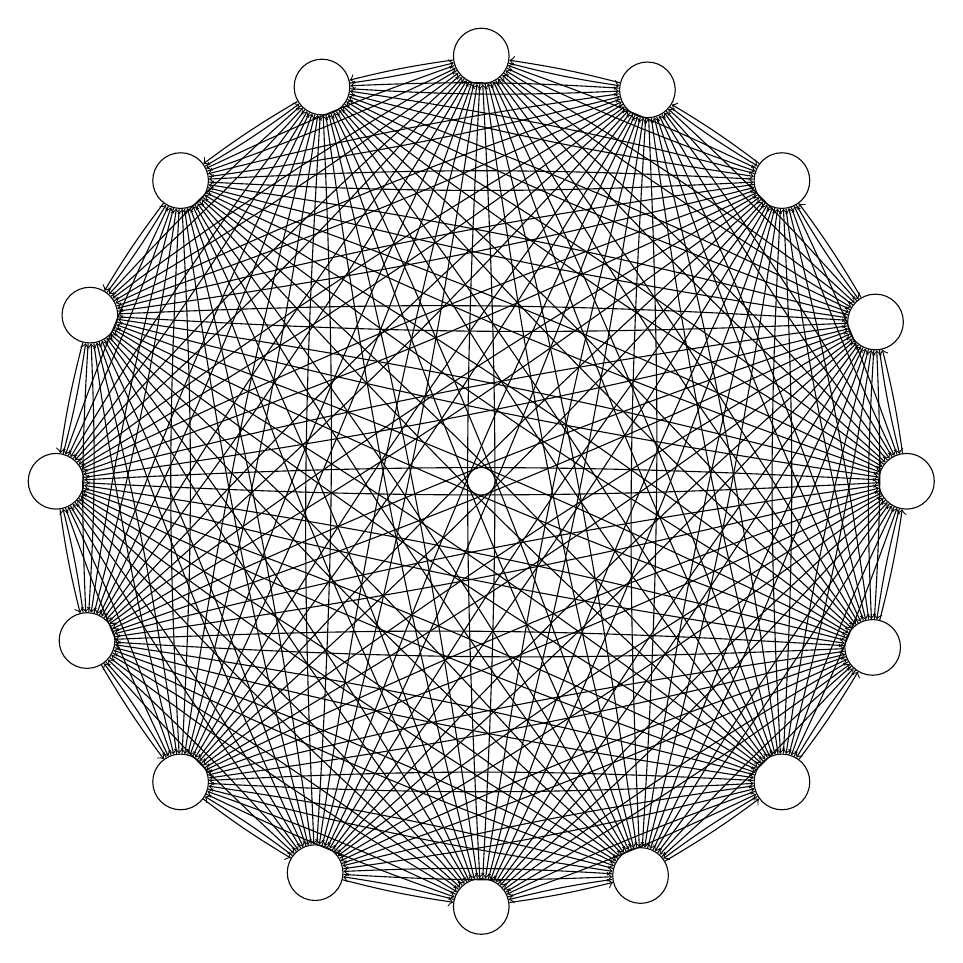
\begin{tikzpicture}[transform shape]
  %the multiplication with floats is not possible. Thus I split the loop in two.
  \foreach \number in {1,...,8}{
      % Computer angle:
        \mycount=\number
        \advance\mycount by -1
  \multiply\mycount by 45
        \advance\mycount by 0
      \node[draw,circle,inner sep=0.25cm] (N-\number) at (\the\mycount:5.4cm) {};
    }
  \foreach \number in {9,...,16}{
      % Computer angle:
        \mycount=\number
        \advance\mycount by -1
  \multiply\mycount by 45
        \advance\mycount by 22.5
      \node[draw,circle,inner sep=0.25cm] (N-\number) at (\the\mycount:5.4cm) {};
    }
  \foreach \number in {1,...,15}{
        \mycount=\number
        \advance\mycount by 1
  \foreach \numbera in {\the\mycount,...,16}{
    \path (N-\number) edge[->,bend right=3] (N-\numbera)  edge[<-,bend
      left=3] (N-\numbera);
  }
}
\end{tikzpicture}

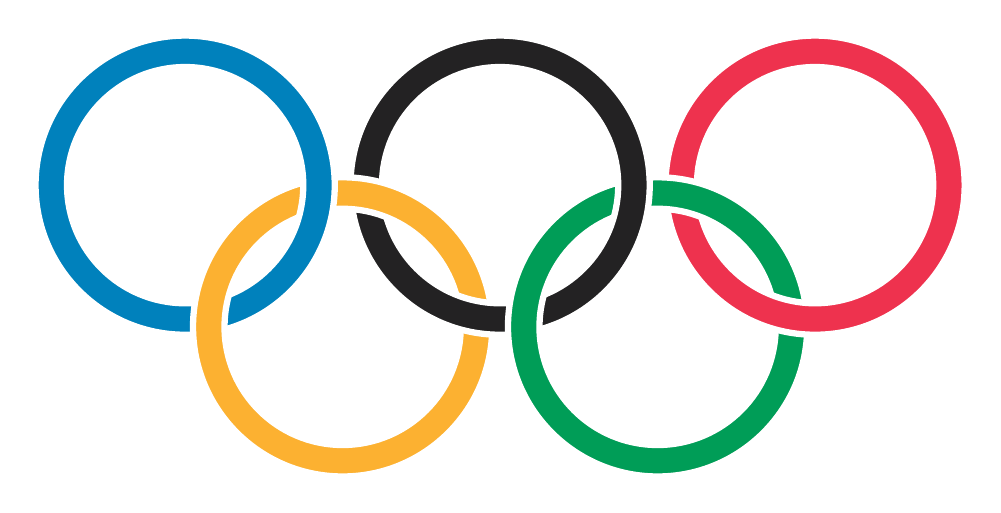
\begin{tikzpicture}
 \definecolor{r1}{RGB}{0,129,188}
 \definecolor{r2}{RGB}{252,177,49}
 \definecolor{r3}{RGB}{35,34,35}
 \definecolor{r4}{RGB}{0,157,87}
 \definecolor{r5}{RGB}{238,50,78}
 \begin{scope}
   \clip (-6,2) rectangle (6,-.9);
   \foreach \col/\xp/\yp in {
     r5/4/0, r4/2/-1.8, r3/0/0,
     r2/-2/-1.8, r1/-4/0
   } {
     \path[draw=white,line width=.08cm,
     fill=\col,even odd rule]
     (\xp, \yp) circle (1.9cm)
     (\xp, \yp) circle (1.5cm);
   }
 \end{scope}
 \begin{scope}
   \clip (-6,-.9) rectangle (6,-3.8);
   \foreach \col/\xp/\yp in {
     r1/-4/0, r2/-2/-1.8, r3/0/0,
     r4/2/-1.8, r5/4/0
   } {
     \path[draw=white,line width=.08cm,
     fill=\col,even odd rule]
     (\xp, \yp) circle (1.9cm)
     (\xp, \yp) circle (1.5cm);
   }
 \end{scope}
\end{tikzpicture}


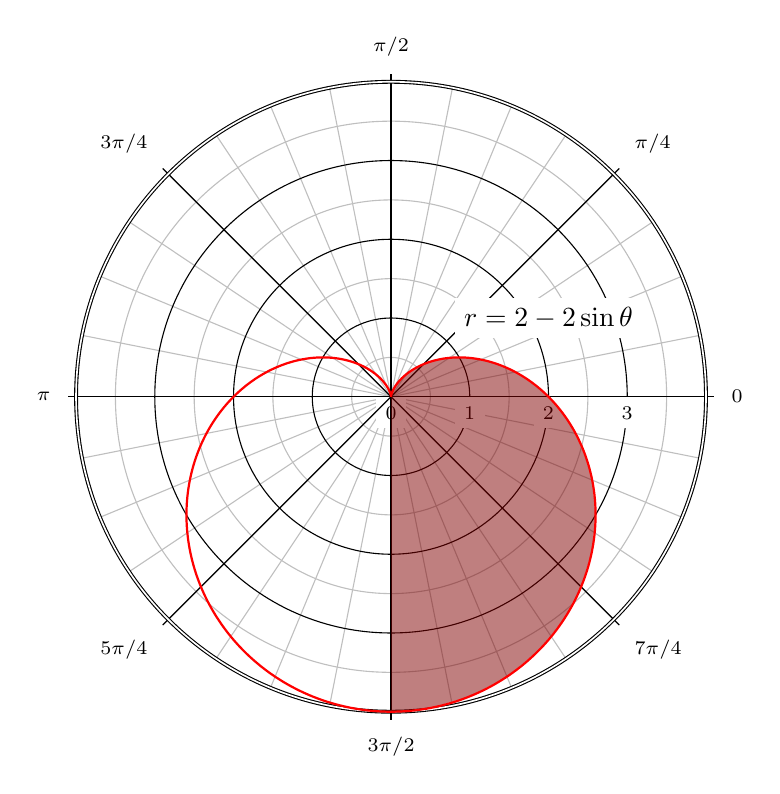
\begin{tikzpicture}[>=latex]

% Draw the lines at multiples of pi/12
\foreach \ang in {0,...,31} {
  \draw [lightgray] (0,0) -- (\ang * 180 / 16:4);
}

% Concentric circles and radius labels
\foreach \s in {0, 1, 2, 3} {
  \draw [lightgray] (0,0) circle (\s + 0.5);
  \draw (0,0) circle (\s);
  \node [fill=white] at (\s, 0) [below] {\scriptsize $\s$};
}

% Add the labels at multiples of pi/4
\foreach \ang/\lab/\dir in {
  0/0/right,
  1/{\pi/4}/{above right},
  2/{\pi/2}/above,
  3/{3\pi/4}/{above left},
  4/{\pi}/left,
  5/{5\pi/4}/{below left},
  7/{7\pi/4}/{below right},
  6/{3\pi/2}/below} {
  \draw (0,0) -- (\ang * 180 / 4:4.1);
  \node [fill=white] at (\ang * 180 / 4:4.2) [\dir] {\scriptsize $\lab$};
}

% The double-lined circle around the whole diagram
\draw [style=double] (0,0) circle (4);

\fill [fill=red!50!black, opacity=0.5] plot [domain=-pi/2:pi/2]
  (xy polar cs:angle=\x r, radius= {2-2*sin(\x r)});
\draw [thick, color=red, domain=0:2*pi, samples=200, smooth]
  plot (xy polar cs:angle=\x r, radius={2-2*sin(\x r)});
\node [fill=white] at (2,1) {$r=2-2\sin\theta$};

\end{tikzpicture} 


% definition de partial ellipse
\tikzset{partial ellipse/.style args =
  {#1:#2:#3}{insert path={+ (#1:#3) arc (#1:#2:#3)}}}
\begin{tikzpicture}[>=latex]
  %  ellipses
  \draw [fill=white!90!red]    (3,-1.8) ellipse    (4cm and 1 cm);
  \draw [fill=yellow!90!green] (3,-1.8) ellipse (3cm and 0.75 cm);
  \draw [fill=white!90!green]  (3,-1.8) ellipse  (2cm and 0.5 cm);

  % -- Soleil
  \shade [ball color=gray!10!yellow] (3,-1.8) circle (1);
  \node (soleil) at (3,-1.8) {\bf Soleil};
  % partial ellipse pour tracé devant le Soleil
  \draw (3,-1.8) [partial ellipse=220:320:2cm and 0.5cm]
        (3,-1.8) [partial ellipse=220:320:3cm and 0.75cm];

  % Venus
  \shade [ball color=gray!10!orange] (1.6,-1.8) circle (.2);
  \node (venus) at (1.5,-1.45) {Venus}; 

  % ombre de Venus
  \draw[color=white!70!black,fill=white!70!black]
    (1.6,-2.3) ellipse (2mm and 0.5mm);

  % Mercure
  \shade [ball color=gray!10!orange] (5,-1.225) circle (.25);
  \node (mercure) at (5,-0.8) {Mercure}; 

  % Earth
  \shade [ball color=white!50!blue] (5.75,-2.5) circle (.33);
  \node (terre) at (6.6,-2.6) {\bf Terre};

  % Lune
  \shade [ball color=yellow] (5.25,-2.8) circle (.1);
  \node (lune) at (5.25,-3) {Lune};
     
  % Mars
  \draw (3,-1.8) [partial ellipse=45:120:9cm and 2.5cm];
  \shade [ball color=black!50!red] (5,0.66) circle (.15);
  \node (mars) at (5,1) {\bf Mars};   
  % trajet
  \draw [line width=2pt,blue,->,>=latex] (terre) to[out=0,in=0] (mars);   
\end{tikzpicture}
\end{center}


\end{document}
